\documentclass[conference]{IEEEtran}
\IEEEoverridecommandlockouts
% The preceding line is only needed to identify funding in the first footnote. If that is unneeded, please comment it out.
\usepackage{cite}
\usepackage{amsmath,amssymb,amsfonts}
\usepackage{algorithmic}
\usepackage{graphicx}
\usepackage{textcomp}
\usepackage{xcolor}
\usepackage{ctex}
\usepackage{fontspec}
\usepackage{listings}
\usepackage{pxfonts}
% The following code is for matlab language
\lstset{
    columns=fixed,     
    basicstyle = \tt,           % 基本样式 + 小号字体  
    %numbers=left,    % 在左侧显示行号
    frame=none,     % 不显示背景边框
    breaklines = true,                  % 代码过长则换行
    backgroundcolor=\color[RGB]{245,245,244},  % 设定背景颜色
    keywordstyle=\color[RGB]{40,40,255},         % 设定关键字颜色
    % numberstyle=\footnotesize\color{darkgray},    % 设定行号格式
    commentstyle=\it\color[RGB]{0,96,96},         % 设置代码注释的格式
    stringstyle=\rmfamily\slshape\color[RGB]{128,0,0},   % 设置字符串格式
    showstringspaces=false,   % 不显示字符串中的空格
    language=matlab,             % 设置语言
    extendedchars=false,
    %basicstyle=Consolas
    tabsize=4,
    upquote=true,
    %literate={'}{\textquotedb}1
}

\def\BibTeX{{\rm B\kern-.05em{\sc i\kern-.025em b}\kern-.08em
    T\kern-.1667em\lower.7ex\hbox{E}\kern-.125emX}}
\begin{document}

\title{傅立叶变换光谱测量技术实验报告}

\author{
    \IEEEauthorblockN{
        黄润华}
        \IEEEauthorblockA{
            \textit{Ocean University of China} \\
            \textit{email@noreply.com}
    \and
    \IEEEauthorblockN{
        杨超}
        \IEEEauthorblockA{
            \textit{Ocean University of China} \\
            \textit{email@somewhere.com}
        }
    }
}




\maketitle

\begin{abstract}
    本实验报告为傅立叶变换光谱测量技术第四次实验报告,本报告采用Python仿真同时考虑有限扫描长度和采样间隔误差两因素影响下的傅里叶变换光谱测量系统的光谱测量曲线。实验仿真误差选取是随机、线性或正弦变化的误差,仿真采样间隔为79.1nm。本仿真以632.8nm的HeNe激光和532nm的YAG激光为例。
\end{abstract}

\begin{IEEEkeywords}
    Optical spectrum, python, fft
\end{IEEEkeywords}

\section{实验目的}
\begin{itemize}
    \item[1.] 思考并仿真扫描长度误差对傅里叶变换光谱测量曲线的影响;
    \item[2.] 思考并仿真采样间隔误差对傅里叶变换光谱测量曲线的影响;
    \item[3.] 学习利用Python仿真不同影响条件下光谱测量曲线。 
\end{itemize} 

\section{实验原理}
\subsection{分辨率和分辨能力}
光谱仪的光谱分辨率是其定性区分彼此非常接近的两个光谱峰的能力的量度。 通常,光谱分辨率由仪器线形状(ILS)的半峰全宽(FWHM)表示,光谱仪的输出光谱具有纯单色输入辐射。

光谱分辨率R由下式定义
\begin{align}
    R = \frac{\sigma_{max}}{\delta \sigma}
\end{align}
其中$\sigma_{max}$是光谱仪设计运行的最大波数。

\subsubsection{分辨率与最大OPD之间的关系}
根据公式
\begin{align}
    B_{c}(\sigma)=B_{r e L}(\sigma)+i B_{i o L}(\sigma)=\int_{-\infty}^{\infty} I(x) \operatorname{rect}(x) e^{-i 2 \pi a x} d x \\
    \begin{cases}{c}
        B(\sigma)=2 \mid \int_{-\infty}^{+\infty} I(x) \operatorname{rect}(x) e^{-2 \pi a x} d x \\
        \phi(\sigma)=\arctan \left[\frac{B_{i o L}(\sigma)}{B_{r e L}(\sigma)}\right]
    \end{cases} \quad(\sigma \geq 0)
\end{align}
其中矩形函数定义为
\begin{align*}
    \operatorname{rect}(x)=\begin{cases}
        1 & |x|<L \\
        0 & |x|>L
        \end{cases}
\end{align*}
因此,理论上 FTS 的光谱分辨率取决于可移动镜的扫描范围
\begin{align}
    B_{e}(\sigma)=\begin{cases}{ll}
        B(\sigma) / 2 & (\sigma \geq 0) \\
        B(-\sigma) / 2 & (\sigma \leq 0)
        \end{cases}
\end{align}
理论上,完美单色线的干涉图可以用来描述
\begin{align}
    I(x) = 2cos(2\pi \sigma_0 x)
\end{align}
将此表达式替换为方程$B(\sigma)$、$\phi(\sigma)$,考虑到实际上$\sigma > 0$,可以得到ILS $B(\sigma)$的表达式:
\begin{align}
        B_{I I S}(\sigma)
        &=2 L\frac{\sin \left[2 \pi\left(\sigma_{0}+\sigma\right) L\right]}{2 \pi\left(\sigma_{0}+\sigma\right) L}+\frac{\sin \left[2 \pi\left(\sigma_{0}-\sigma\right) L\right]}{2 \pi\left(\sigma_{0}-\sigma\right) L} \\
        & \approx 2 L \times \frac{\sin \left[2 \pi\left(\sigma_{0}-\sigma\right) L\right]}{2 \pi\left(\sigma_{0}-\sigma\right) L}  \\
        & =2 L \sin c\left[2 \pi\left(\sigma_{0}-\sigma\right) L\right]
\end{align}
如图\ref{pic8}所示,光谱从一条线($\delta$ 函数)扩展到 $sin c$ 函数形状(仪器线形)。
\begin{align}
    (\delta \sigma)_{linewidth} = \frac{1.21}{2L}
\end{align}

\begin{figure}[htbp]
    \centerline{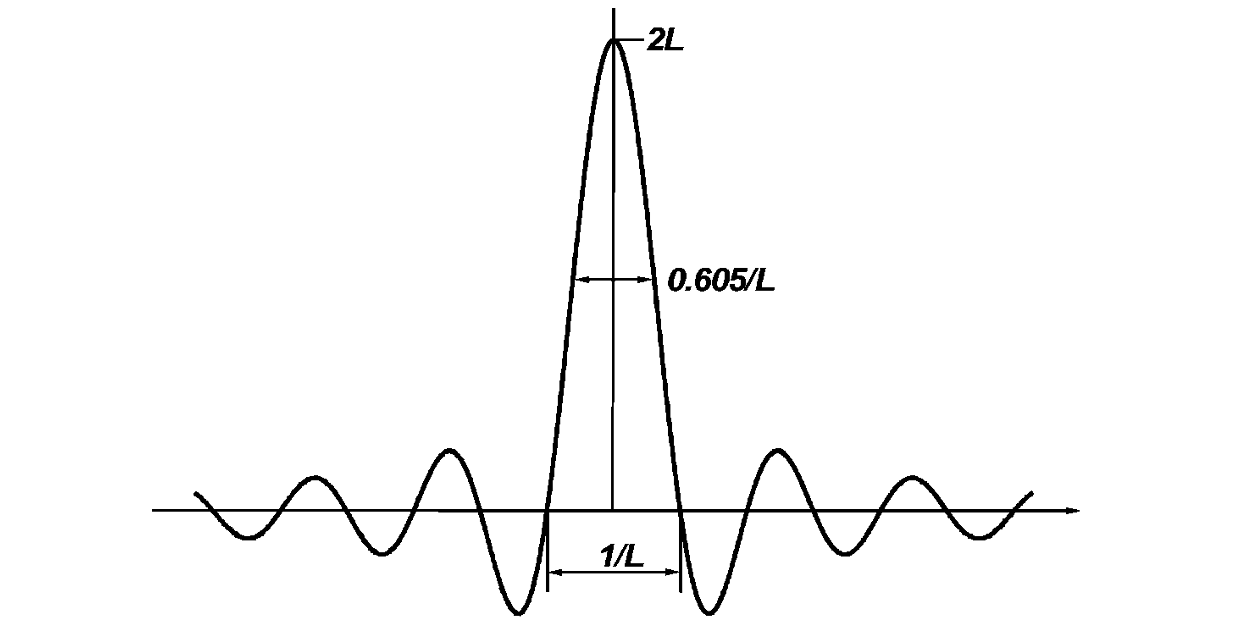
\includegraphics[width=0.5\textwidth]{pic8.png}}
    \caption{$B_{I I S}(\sigma)$}
    \label{pic8}
\end{figure}

\subsubsection{分离共振}
分辨率可以通过分离图\ref{pic9}所示光谱中相同强度(或共振)的两条单色线(波数和)来描述。
如果两个线峰值之间的下降幅度大于线峰值的 20\%,则可以声称解决了两个共振,此时
\begin{align}
    (\delta \sigma)_{separation} = \frac{1.46}{2L}
\end{align}

\begin{figure}[htbp]
    \centerline{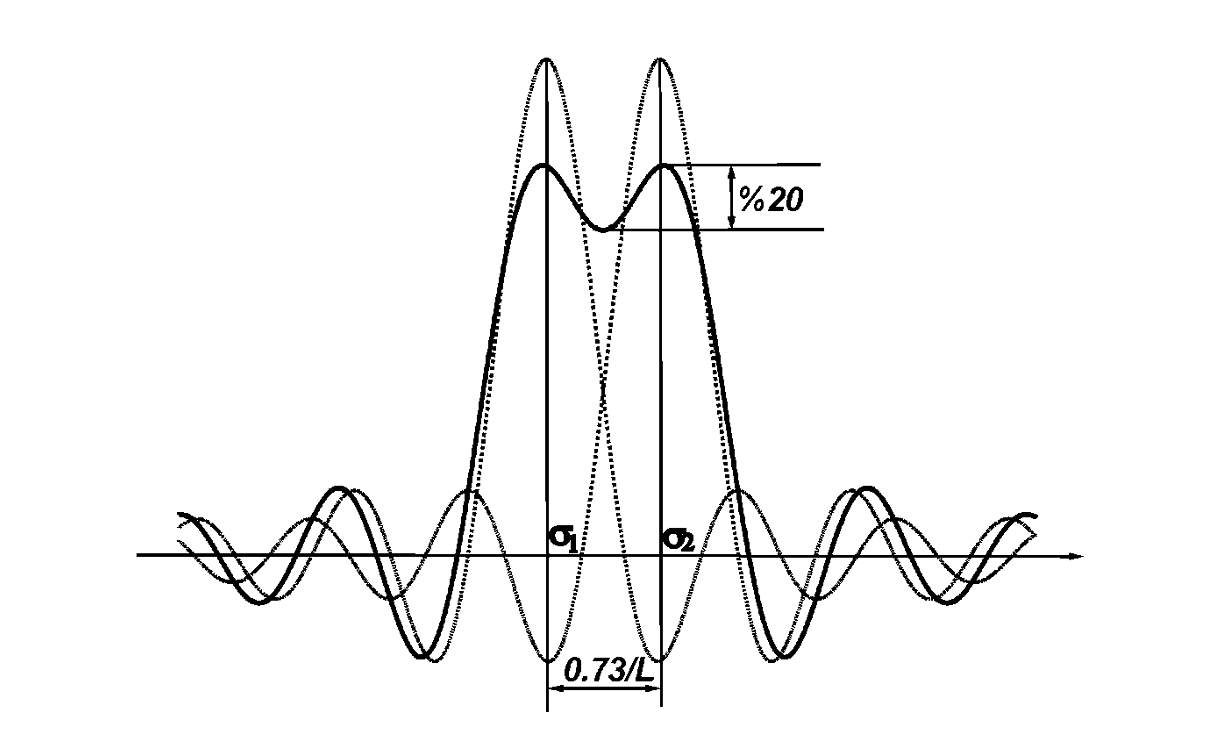
\includegraphics[width=0.5\textwidth]{pic9.png}}
    \caption{分离共振解析结果}
    \label{pic9}
\end{figure}

\subsubsection{瑞利准则}
瑞利准则分离两个 ILS 的峰值,使得一个共振的最大值落在另一个共振的零点处,因此,仪器线形状决定的分辨率是
\begin{align}
    \delta \sigma = \frac{1}{2L}
\end{align} 

\subsection{分辨率与发散角度之间的关系}
图\ref{pic10}是迈克尔逊干涉仪的等效图,根据图\ref{pic10}与图\ref{pic11}可以计算出OPD与夹角$\theta$之间的关系
\begin{align}
    O P D=2 \times \frac{x / 2}{\cos \theta}-x \tan \theta \sin \theta=x \cos \theta
\end{align}

\begin{figure}[htbp]
    \centerline{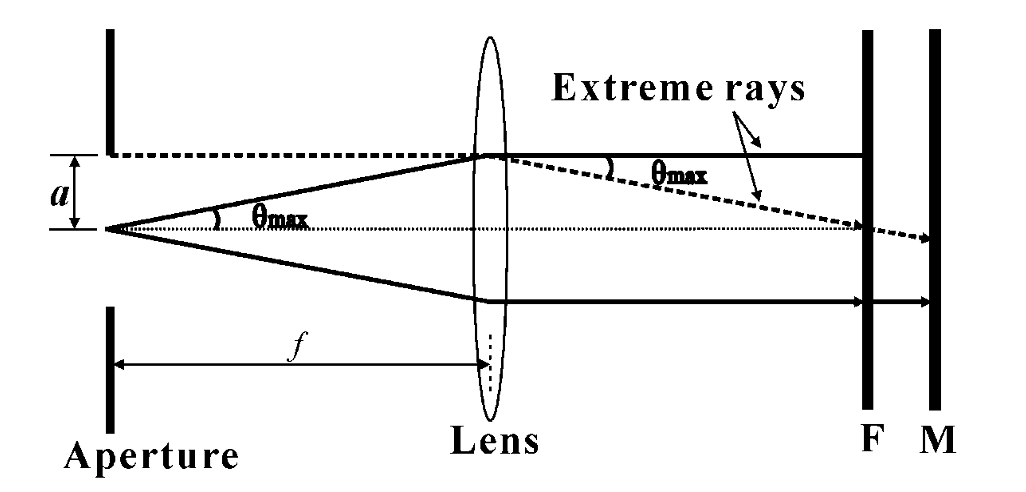
\includegraphics[width=0.5\textwidth]{pic10.png}}
    \caption{迈克尔逊干涉仪的等效图}
    \label{pic10}
\end{figure}

\begin{figure}[htbp]
    \centerline{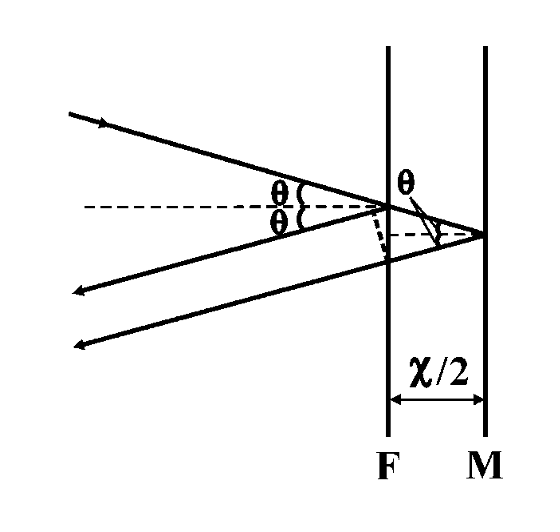
\includegraphics[width=0.5\textwidth]{pic11.png}}
    \caption{迈克尔逊干涉仪接收端放大图}
    \label{pic11}
\end{figure}
我们可以得到扩展源的归一化干涉图,对着一个立体角$\Omega_{max}$是
\begin{align*}
    I\left(x, \Omega_{\max }\right)=\frac{1}{\Omega_{\max }}\int_{0}^{\infty} B(\sigma) \int_{0}^{\Omega_{\operatorname{mix}}} \cos (2 \pi \sigma x \cos \theta) d \Omega d \sigma
\end{align*}
根据立体角的公式,上述式子可以化简为
\begin{align*}
    I\left(x, \Omega_{\max }\right)=\int_{0}^{\infty} B(\sigma) sinc \frac{\Omega_{\max } \sigma x }{2}  &\cos [2 \pi \sigma x\\
    & \;\;\;\;\;\;\;\;\;- \frac{\Omega_{\max } \sigma x }{2}] d \sigma
\end{align*}
对于单色光源其满足
\begin{align*}
    B(\sigma) = \delta(\sigma-\sigma_0)
\end{align*}
其仪器线轮廓可以写为
\begin{align*}
    \begin{cases}
        B_{D i v-1 L S}(\sigma)=[\pi /(\sigma_{0} \Omega_{\max })] \operatorname{rect}(\sigma_{1}, \sigma_{2})\\ \;\;\;\;\;\;\;\;\;\;\;\;\;\;\;\;\;\;\;\;\;\;\;\;\;\;\;\;\;\;\;\;+[\pi /(\sigma_{0} \Omega_{\max })] \operatorname{rect}(-\sigma_{2},-\sigma_{1}) \\
        \sigma_{2}=\sigma_{0}-\sigma_{0} \Omega_{\max } / 2 \pi \\
        \sigma_{1}=\sigma_{0}
    \end{cases}
\end{align*}
于是可以得到
\begin{align}
    &B_{D i v-1 L S}(\sigma)=\left[\pi /\left(\sigma_{0} \Omega_{\max }\right) \operatorname{lrect}\left(\sigma_{1}, \sigma_{2}\right)\right. \\
    &\bar{\sigma}=\sigma_{0}\left[1-\left(\Omega_{\max } / 4 \pi\right)\right]
\end{align}
总的波数差或分辨率是
\begin{align*}
    \delta \sigma = \frac{\sigma_0\Omega_{max}}{2\pi}
\end{align*}
考虑到可移动镜的扫描长度有限,实际 FTS 的 ILS 应该是
\begin{align}
    B_{I L S}(\sigma)=B_{D i v-I L S}(\sigma) * 2 L \sin c[2 \pi \sigma L]
\end{align}
其中$L$是可移动镜的最大位移,$*$是卷积算子。
图\ref{pic11}中两个极端射线的OPD之间的差异公式如下:
\begin{align*}
    \Delta O P D=2 L-2 L \cos \theta_{\max } \approx L \theta_{\max }^{2}=L \frac{a^{2}}{ f^{2}}
\end{align*}
其中$a$是入口孔径的半径,$f$是准直器的焦距。当$\Delta OPD$等于$\lambda/2$时,两条光线异相,它们之
间会发生破坏性叠加。对于宽带辐射输入,存在的最短波长决定了 FTS 的$\Delta OPD$的最大有效值, 如下式所示:
\begin{align}
    \Delta OPD \leq \frac{\lambda_{min}}{2} = \frac{1}{2\sigma_{max}}
\end{align}
我们可以得到 $a$的值应满足以下不等式, 以获得大于$R$的分辨率:
\begin{align}
    a \leq \frac{f}{\sqrt{R}}
\end{align}


\subsection{傅里叶变换光谱仪的优点}
与色散光谱仪相比,FTS具有许多广泛宣传的优点。然而,只有吞吐量(Jacquinot)和多路复用(Felgett)优势是FTS操作原理所固有的,而不是特定的工程设计。
\subsubsection{吞吐量或Jacquinot优势} 吞吐量优势是FTS可以具有大的圆形入口孔,其面积比分散光谱仪中的狭缝的面积大得多,以获得相同的分辨率。吞吐量 定义为 ,其中 是限制孔径的面积,并且是图\ref{pic12}中所示的准直或聚焦光学器件所对应的立体角。

FTS的最大吞吐量由下式给出
\begin{align}
    T_{FTS} = A\Omega_s = \frac{\pi}{R}A_{mirror}
\end{align}
其中$A_{mirror}$是镜子的投影面积。

\begin{figure}[htbp]
    \centerline{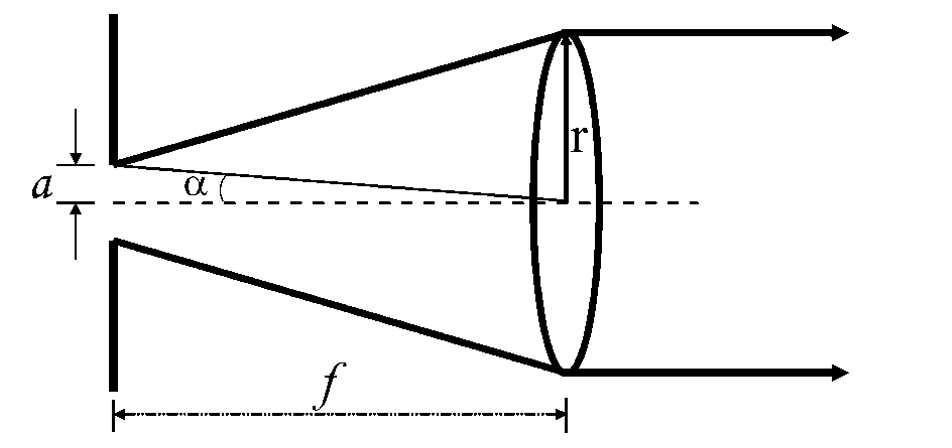
\includegraphics[width=0.5\textwidth]{pic12.png}}
    \caption{孔径和立体角的关系图}
    \label{pic12}
\end{figure}

对于光栅光谱仪,实现分辨率R的能量吞吐量受其狭缝区域和准直光学系统的限制,并由下式给出:
\begin{align}
    T_{grating} = \frac{l}{f_gR}A_{grating}
\end{align}
其中$f_g$是准直光学系统的焦距,$l$是狭缝的高度,$A_{grating}$是光栅的投影面积。对于光栅光谱仪,$\frac{l}{f_gR}$小于1/20。

因此,对于相同的分辨率和类似的仪器尺寸,FTS比光栅光谱仪具有高60倍的能量收集能力。 因此,Jacquinot的优势使得FTS更适合于弱信号测量,其中检测器噪声占主导地位,频谱信噪比(SNR)与吞吐量成比例地增加。

\subsubsection{Multiplex或Felgett的优势} 
多路复用的优点是FTS在扫描周期内同时观察来自给定频谱的整个范围的所有频谱信息。因此,通过使用FTS和使用单色仪可获得的SNR的比率:
\begin{align}
    \frac{SNR^S_{FTS}}{SNR_{monochromator}} = N^{\frac{1}{2}}
\end{align}
FTS的多重优势仅存在于红外和远红外信号的测量中,并且在可见 - 紫外信号的检测中丢失,因为在红外检测中,与信号电平无关的检测器噪声占主导地位。 量子噪声在可见光 - 紫外信号检测中占主导地位。
\subsubsection{Connes的优势}
FTS的波数范围来自He-Ne激光条纹,其作为每次扫描中采样位置的内部参考。 这种激光的波数非常准确,并且非常稳定。 因此,干涉仪的波数校准更精确,并且具有比分散仪器的校准好得多的长期稳定性.


\section{实验内容}
仿真同时考虑有限扫描长度和采样间隔误差两因素影响下的傅里叶变换光谱测量系统的光谱测量曲线。误差可以是随机、线性或正选变化的。以632.8nm的He-Ne激光和532nm的YAG激光为例。(采样间隔为79.1nm)

\begin{figure*}[htbp]
	\centerline{
		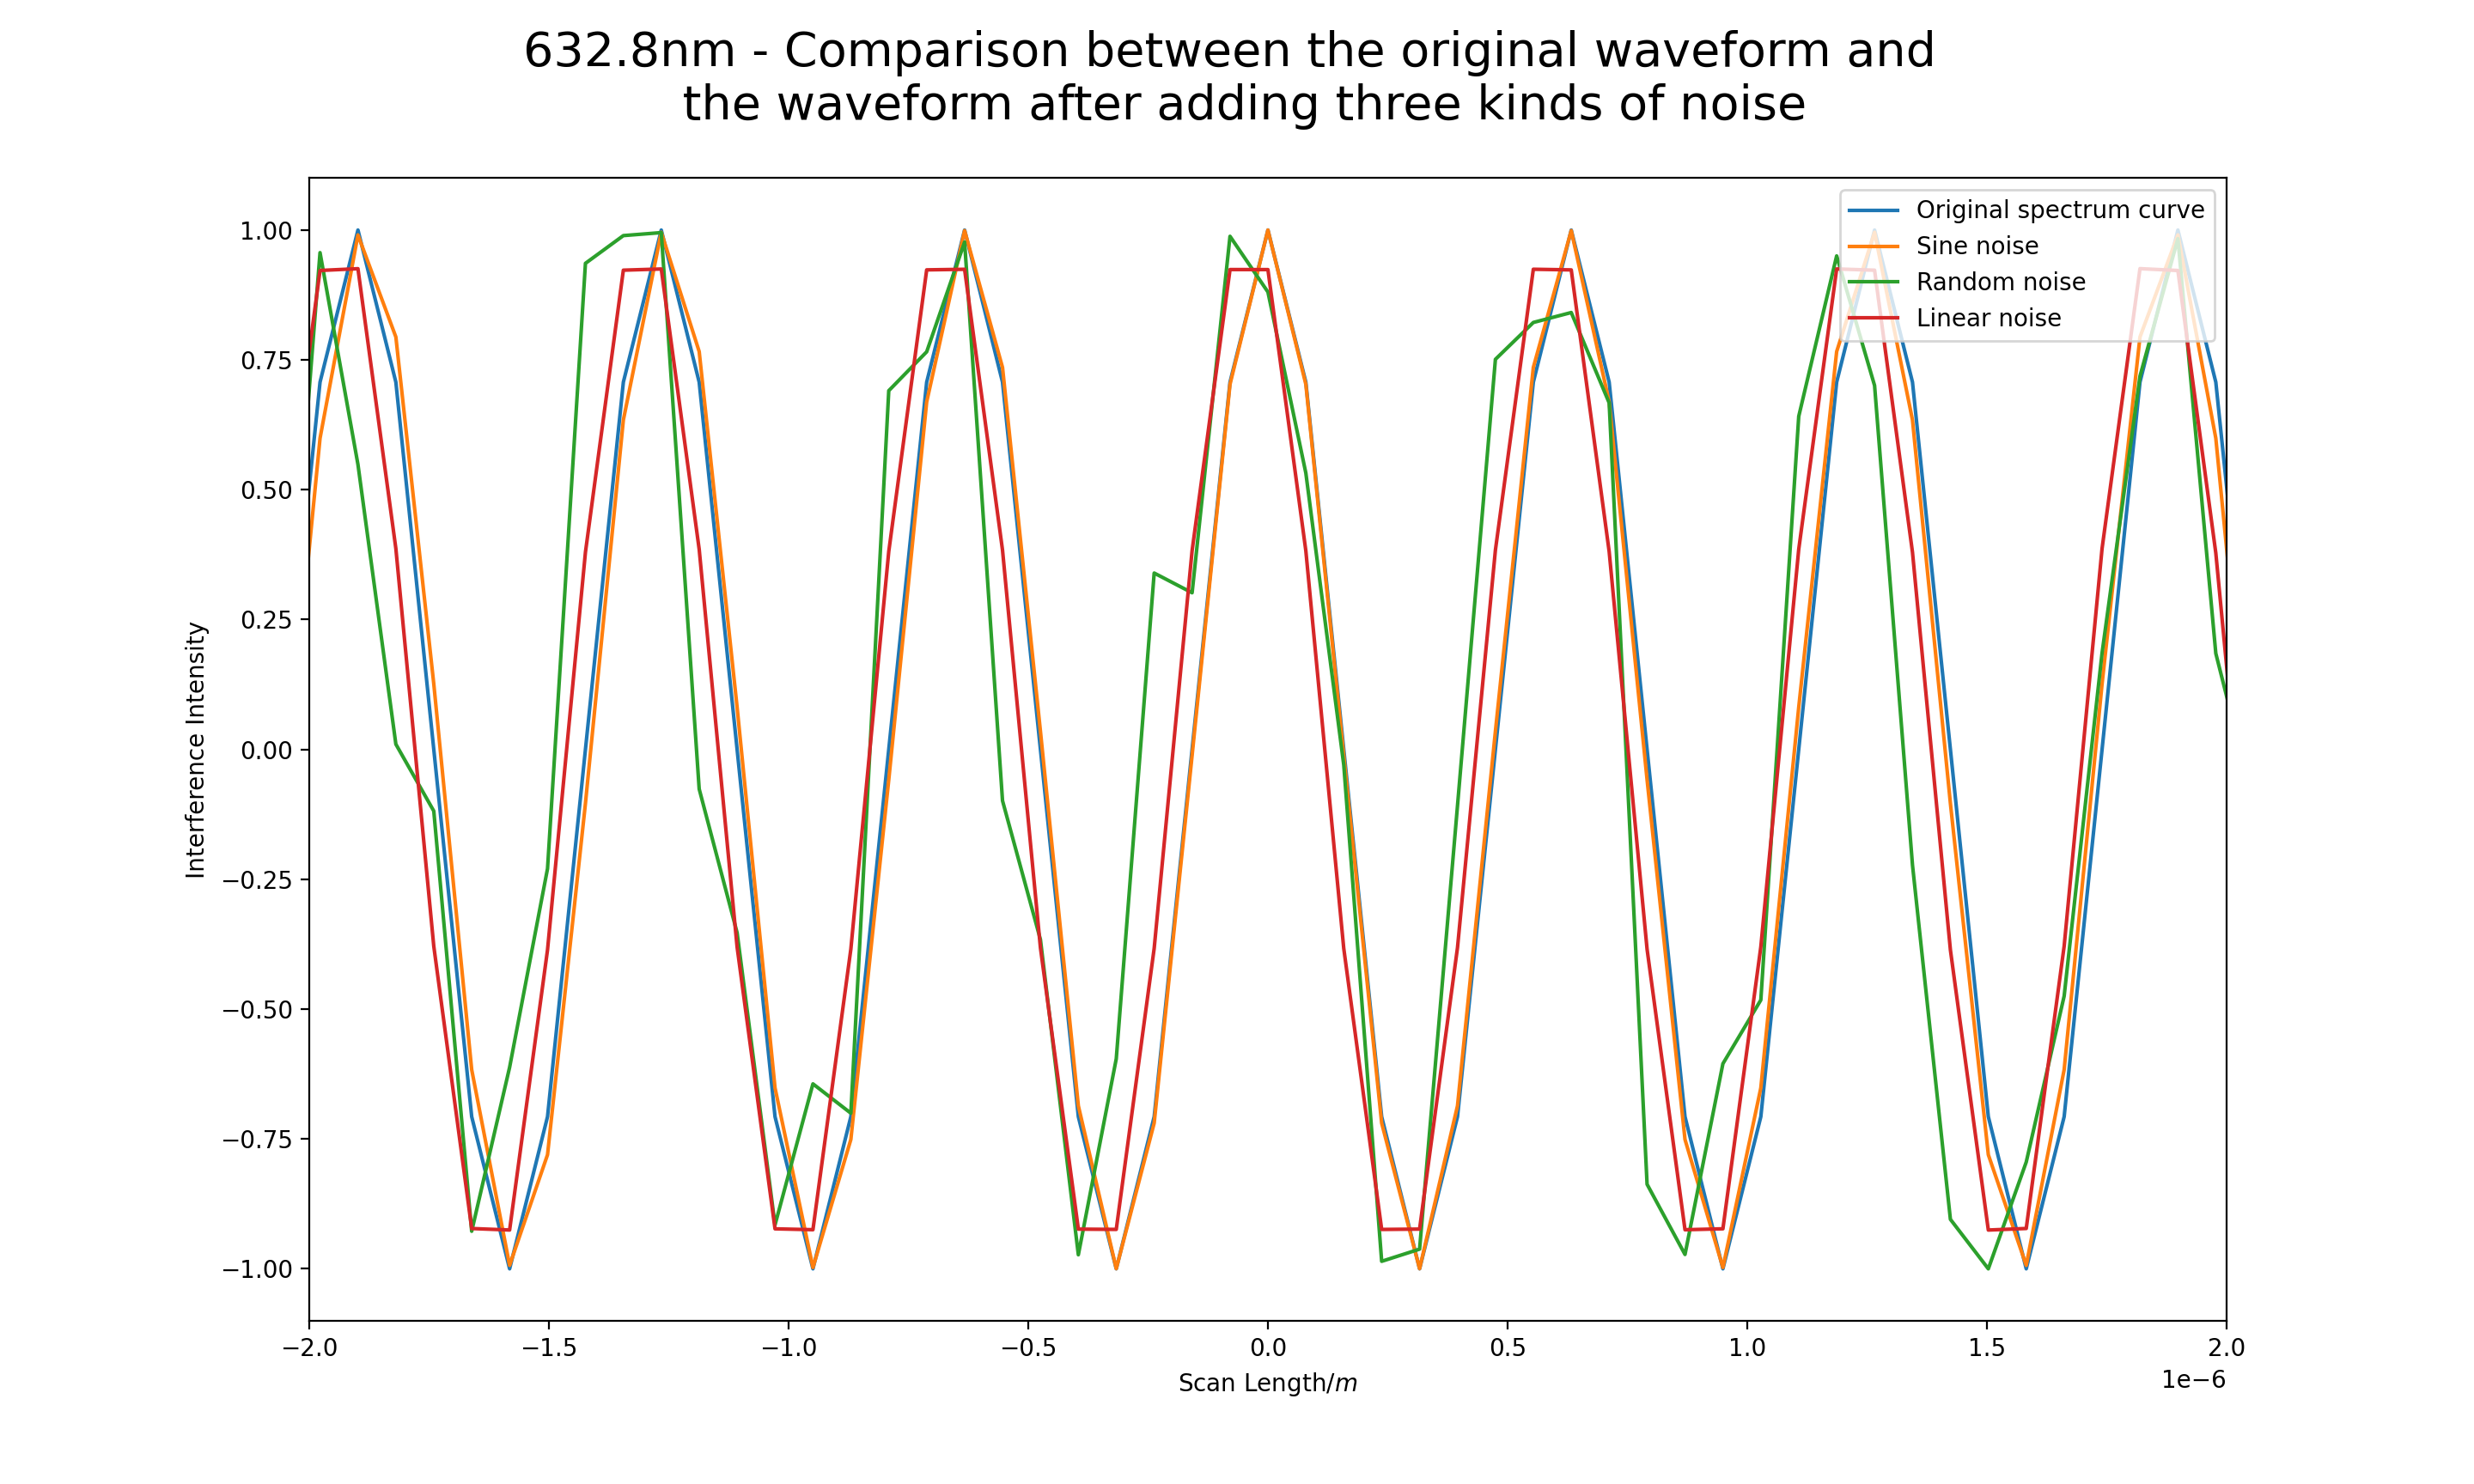
\includegraphics[width=22cm]{pic7.png} 	
	}
	\caption{原始信号的干涉图与叠加三种不同噪声后干涉图的比较}
	\label{pic7}
\end{figure*}

\section{实验结果}
本实验报告以632.8nm的波长为例。
\subsection{三种不同的叠加噪声}
图片\ref{pic1}、图\ref{pic2}与图\ref{pic3}显示了本次仿真的三种不同的叠加噪声,其中图\ref{pic1}为叠加的正弦噪声,图\ref{pic2}为叠加的随机噪声,图\ref{pic3}为叠加的线性噪声。

\begin{figure}[htbp]
    \centerline{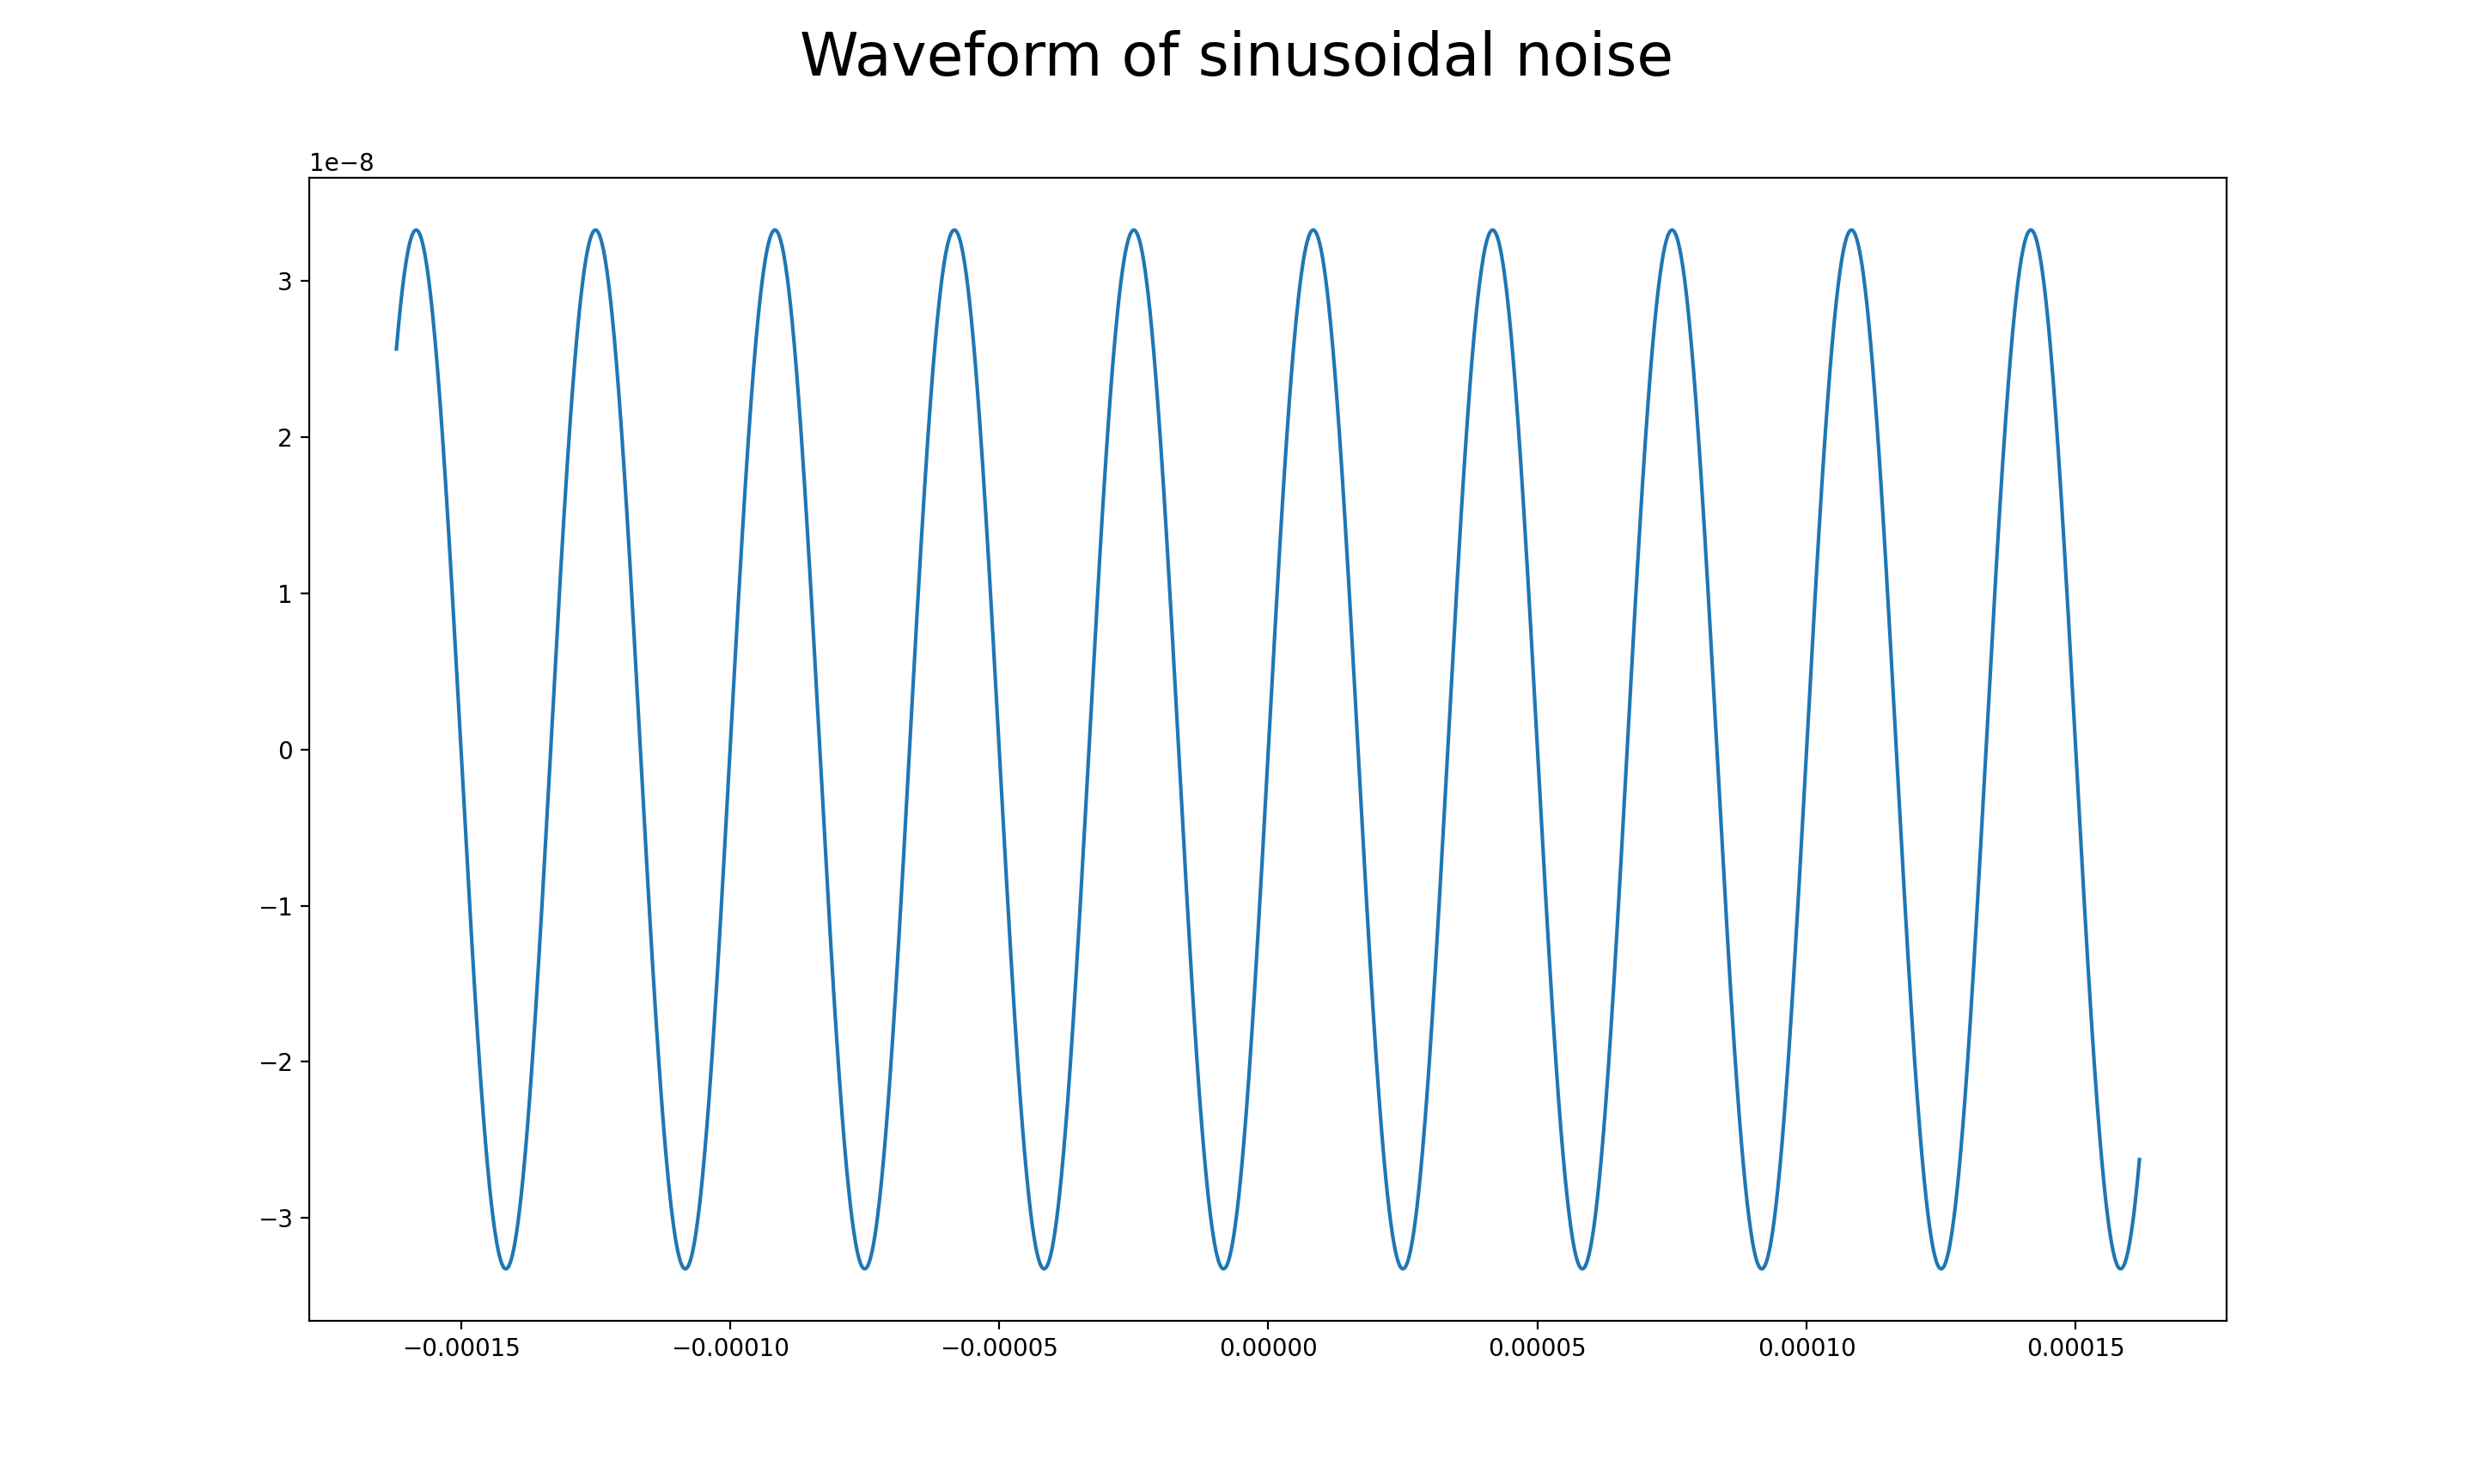
\includegraphics[width=0.5\textwidth]{pic1.png}}
    \caption{叠加的正弦噪声}
    \label{pic1}
\end{figure}

\begin{figure}[htbp]
    \centerline{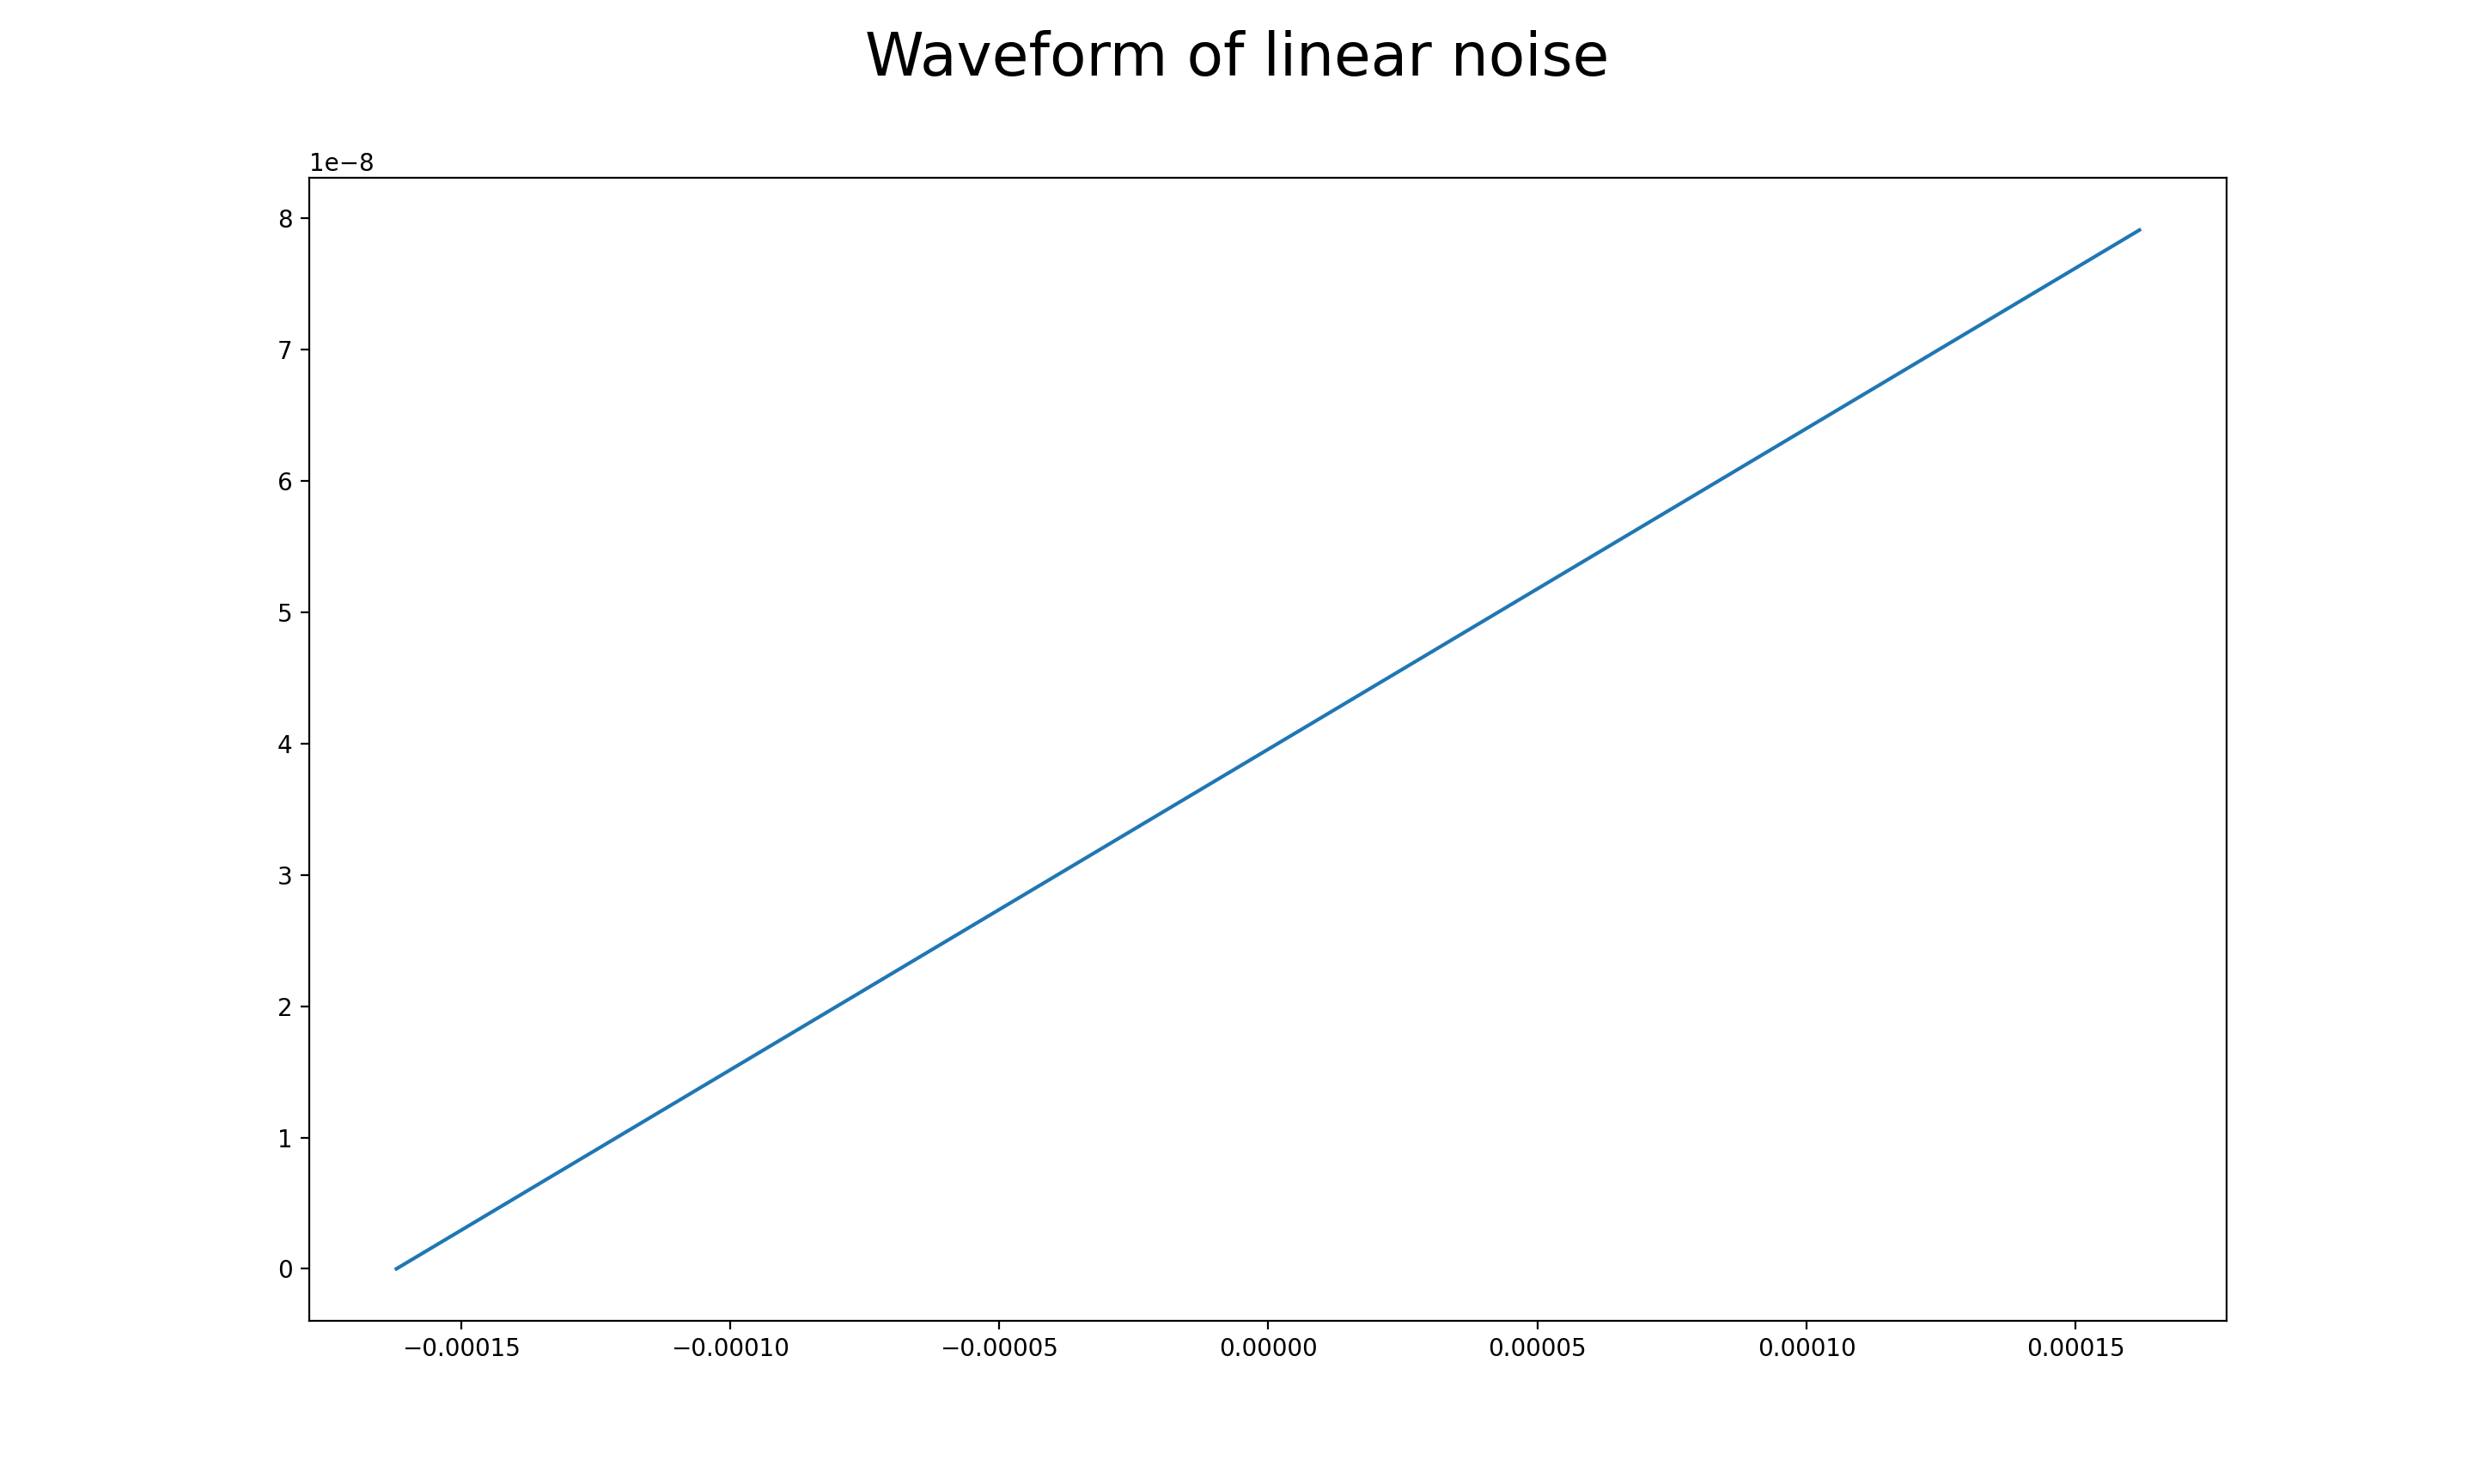
\includegraphics[width=0.5\textwidth]{pic2.png}}
    \caption{叠加的随机噪声}
    \label{pic2}
\end{figure}

\begin{figure}[htbp]
    \centerline{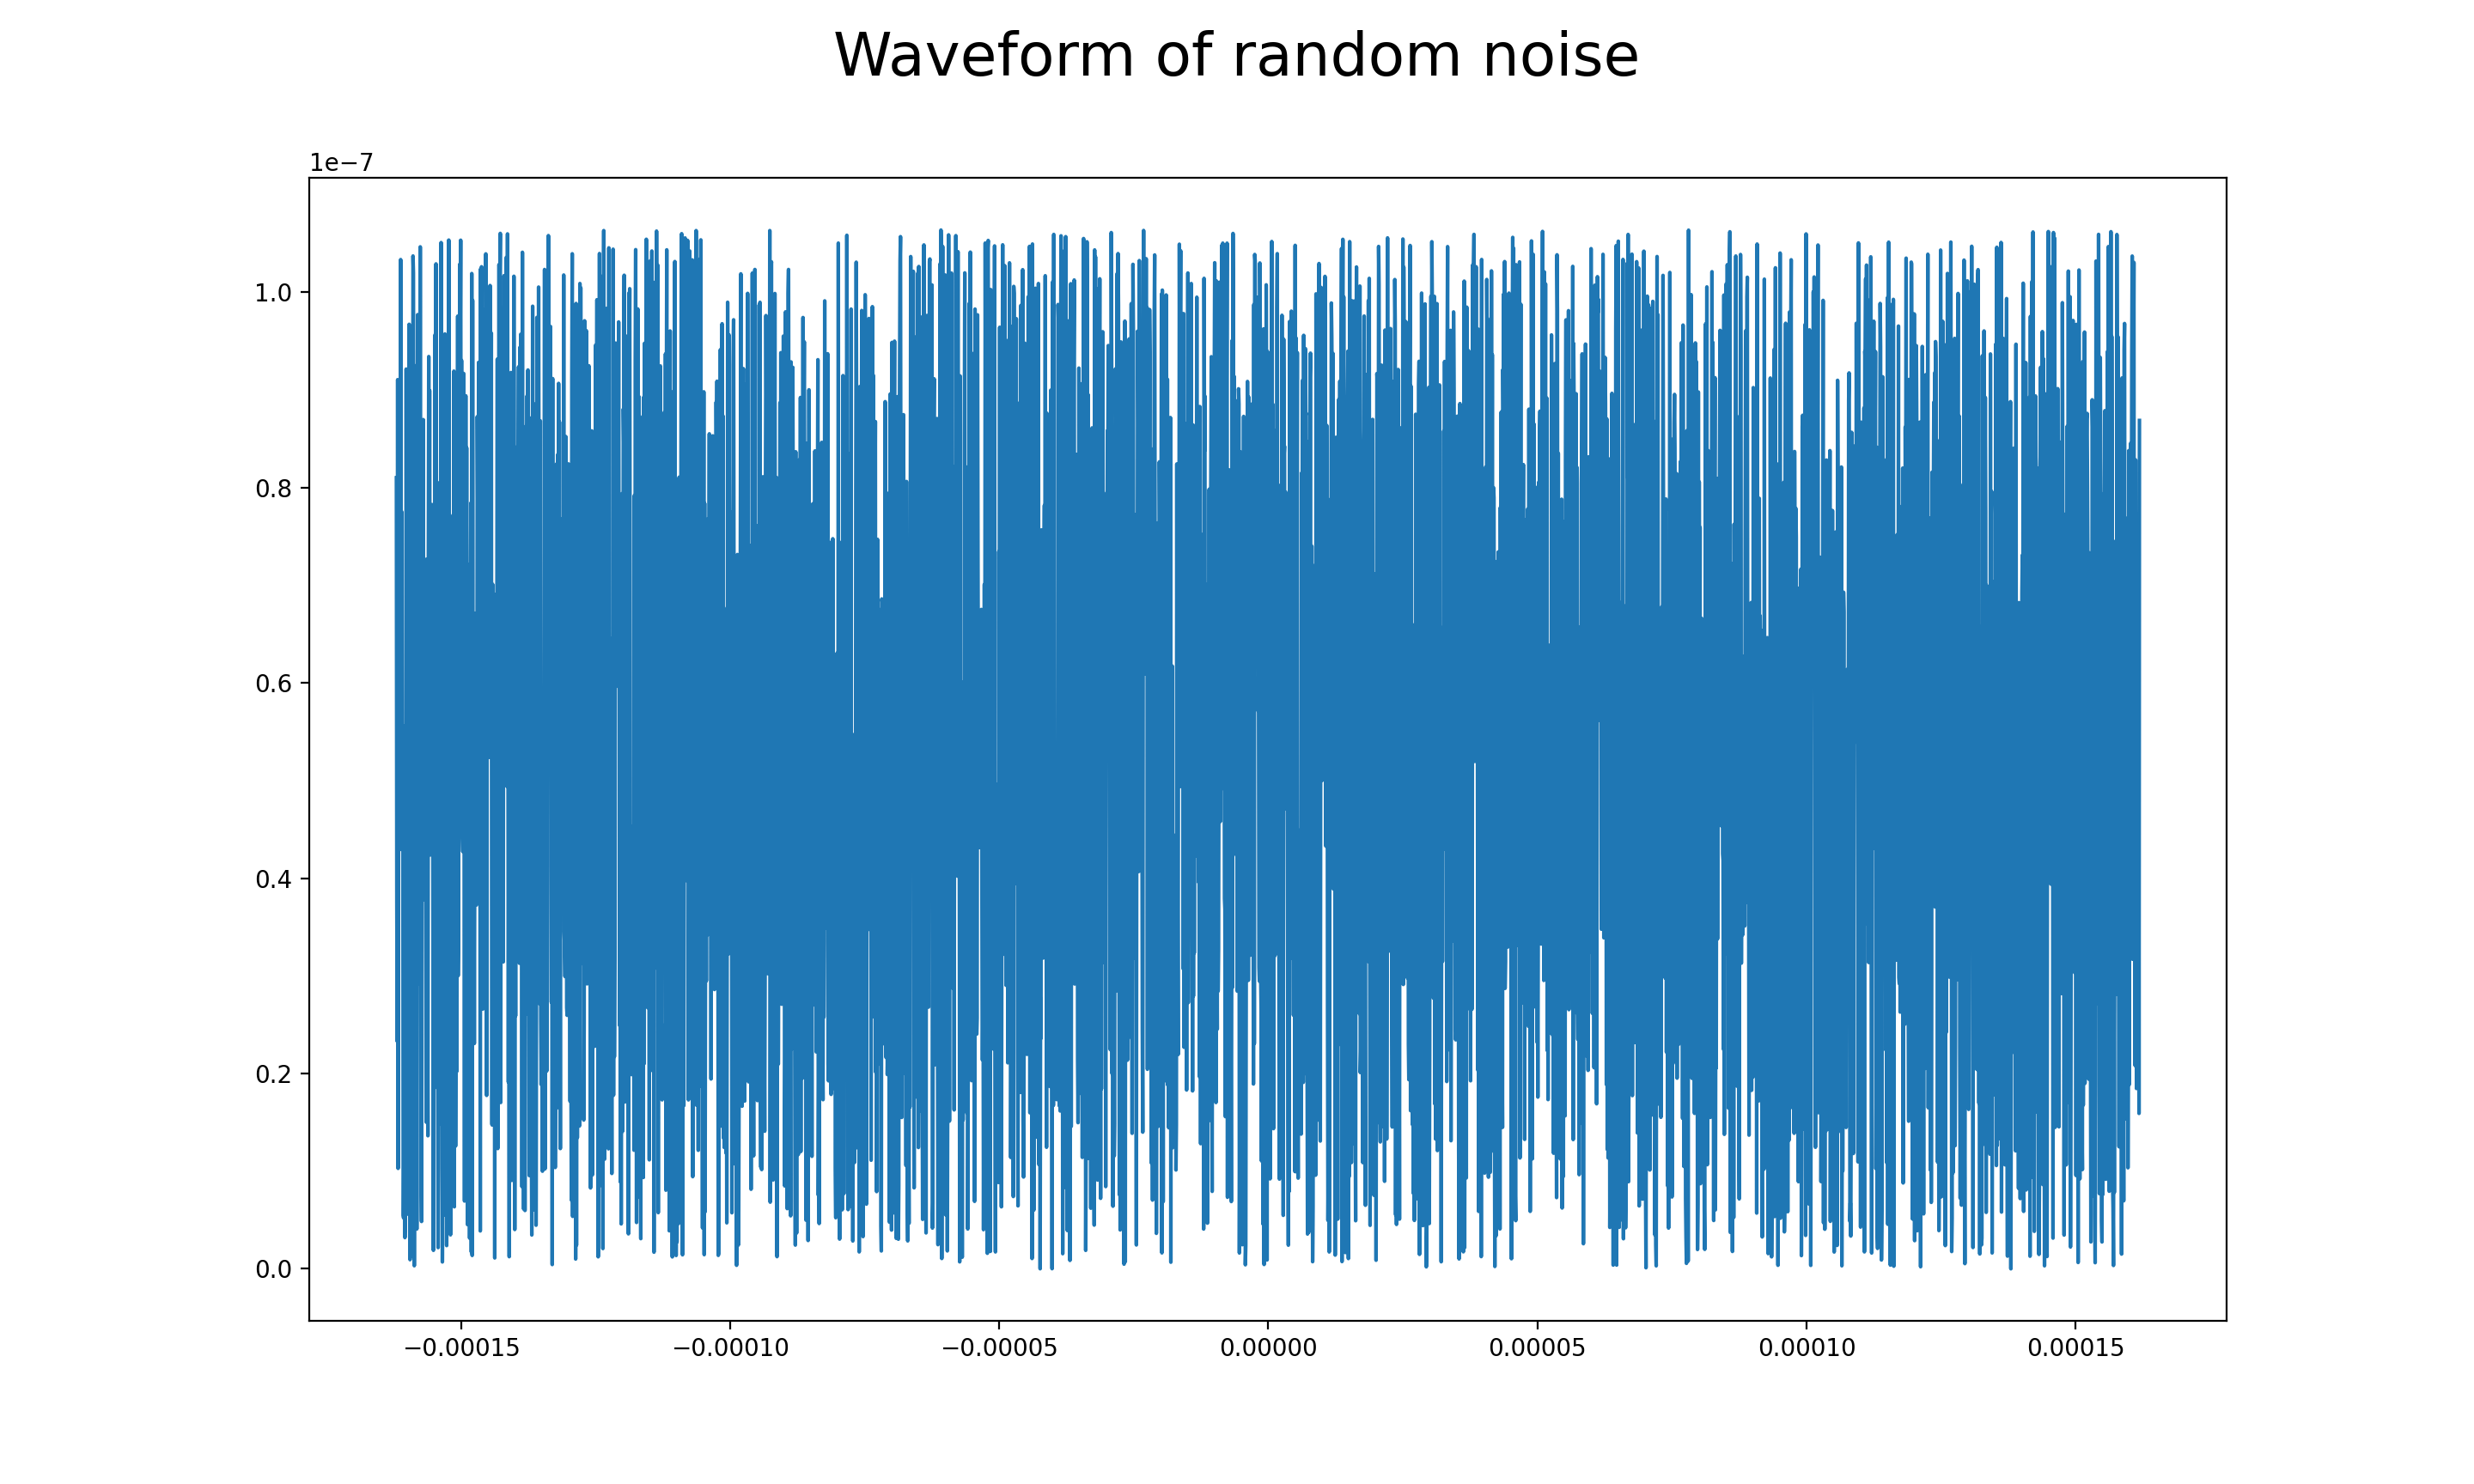
\includegraphics[width=0.5\textwidth]{pic3.png}}
    \caption{叠加的线性噪声}
    \label{pic3}
\end{figure}

\subsection{噪声叠加结果}
图片\ref{pic4}、图\ref{pic5}与图\ref{pic6}显示了三种不同噪声的叠加结果,其中图\ref{pic4}叠加了正弦噪声,图\ref{pic5}叠加了随机噪声,图\ref{pic6}叠加了线性噪声。每张图片第一行代表未叠加噪声的干涉图与光谱曲线图,第二行代表添加部分噪声后的干涉图与光谱曲线图;左半部分代表无噪声干扰与叠加噪声干扰后的干涉图,右半部分代表无噪声干扰与叠加噪声干扰后的光谱曲线图。

\begin{figure}[htbp]
    \centerline{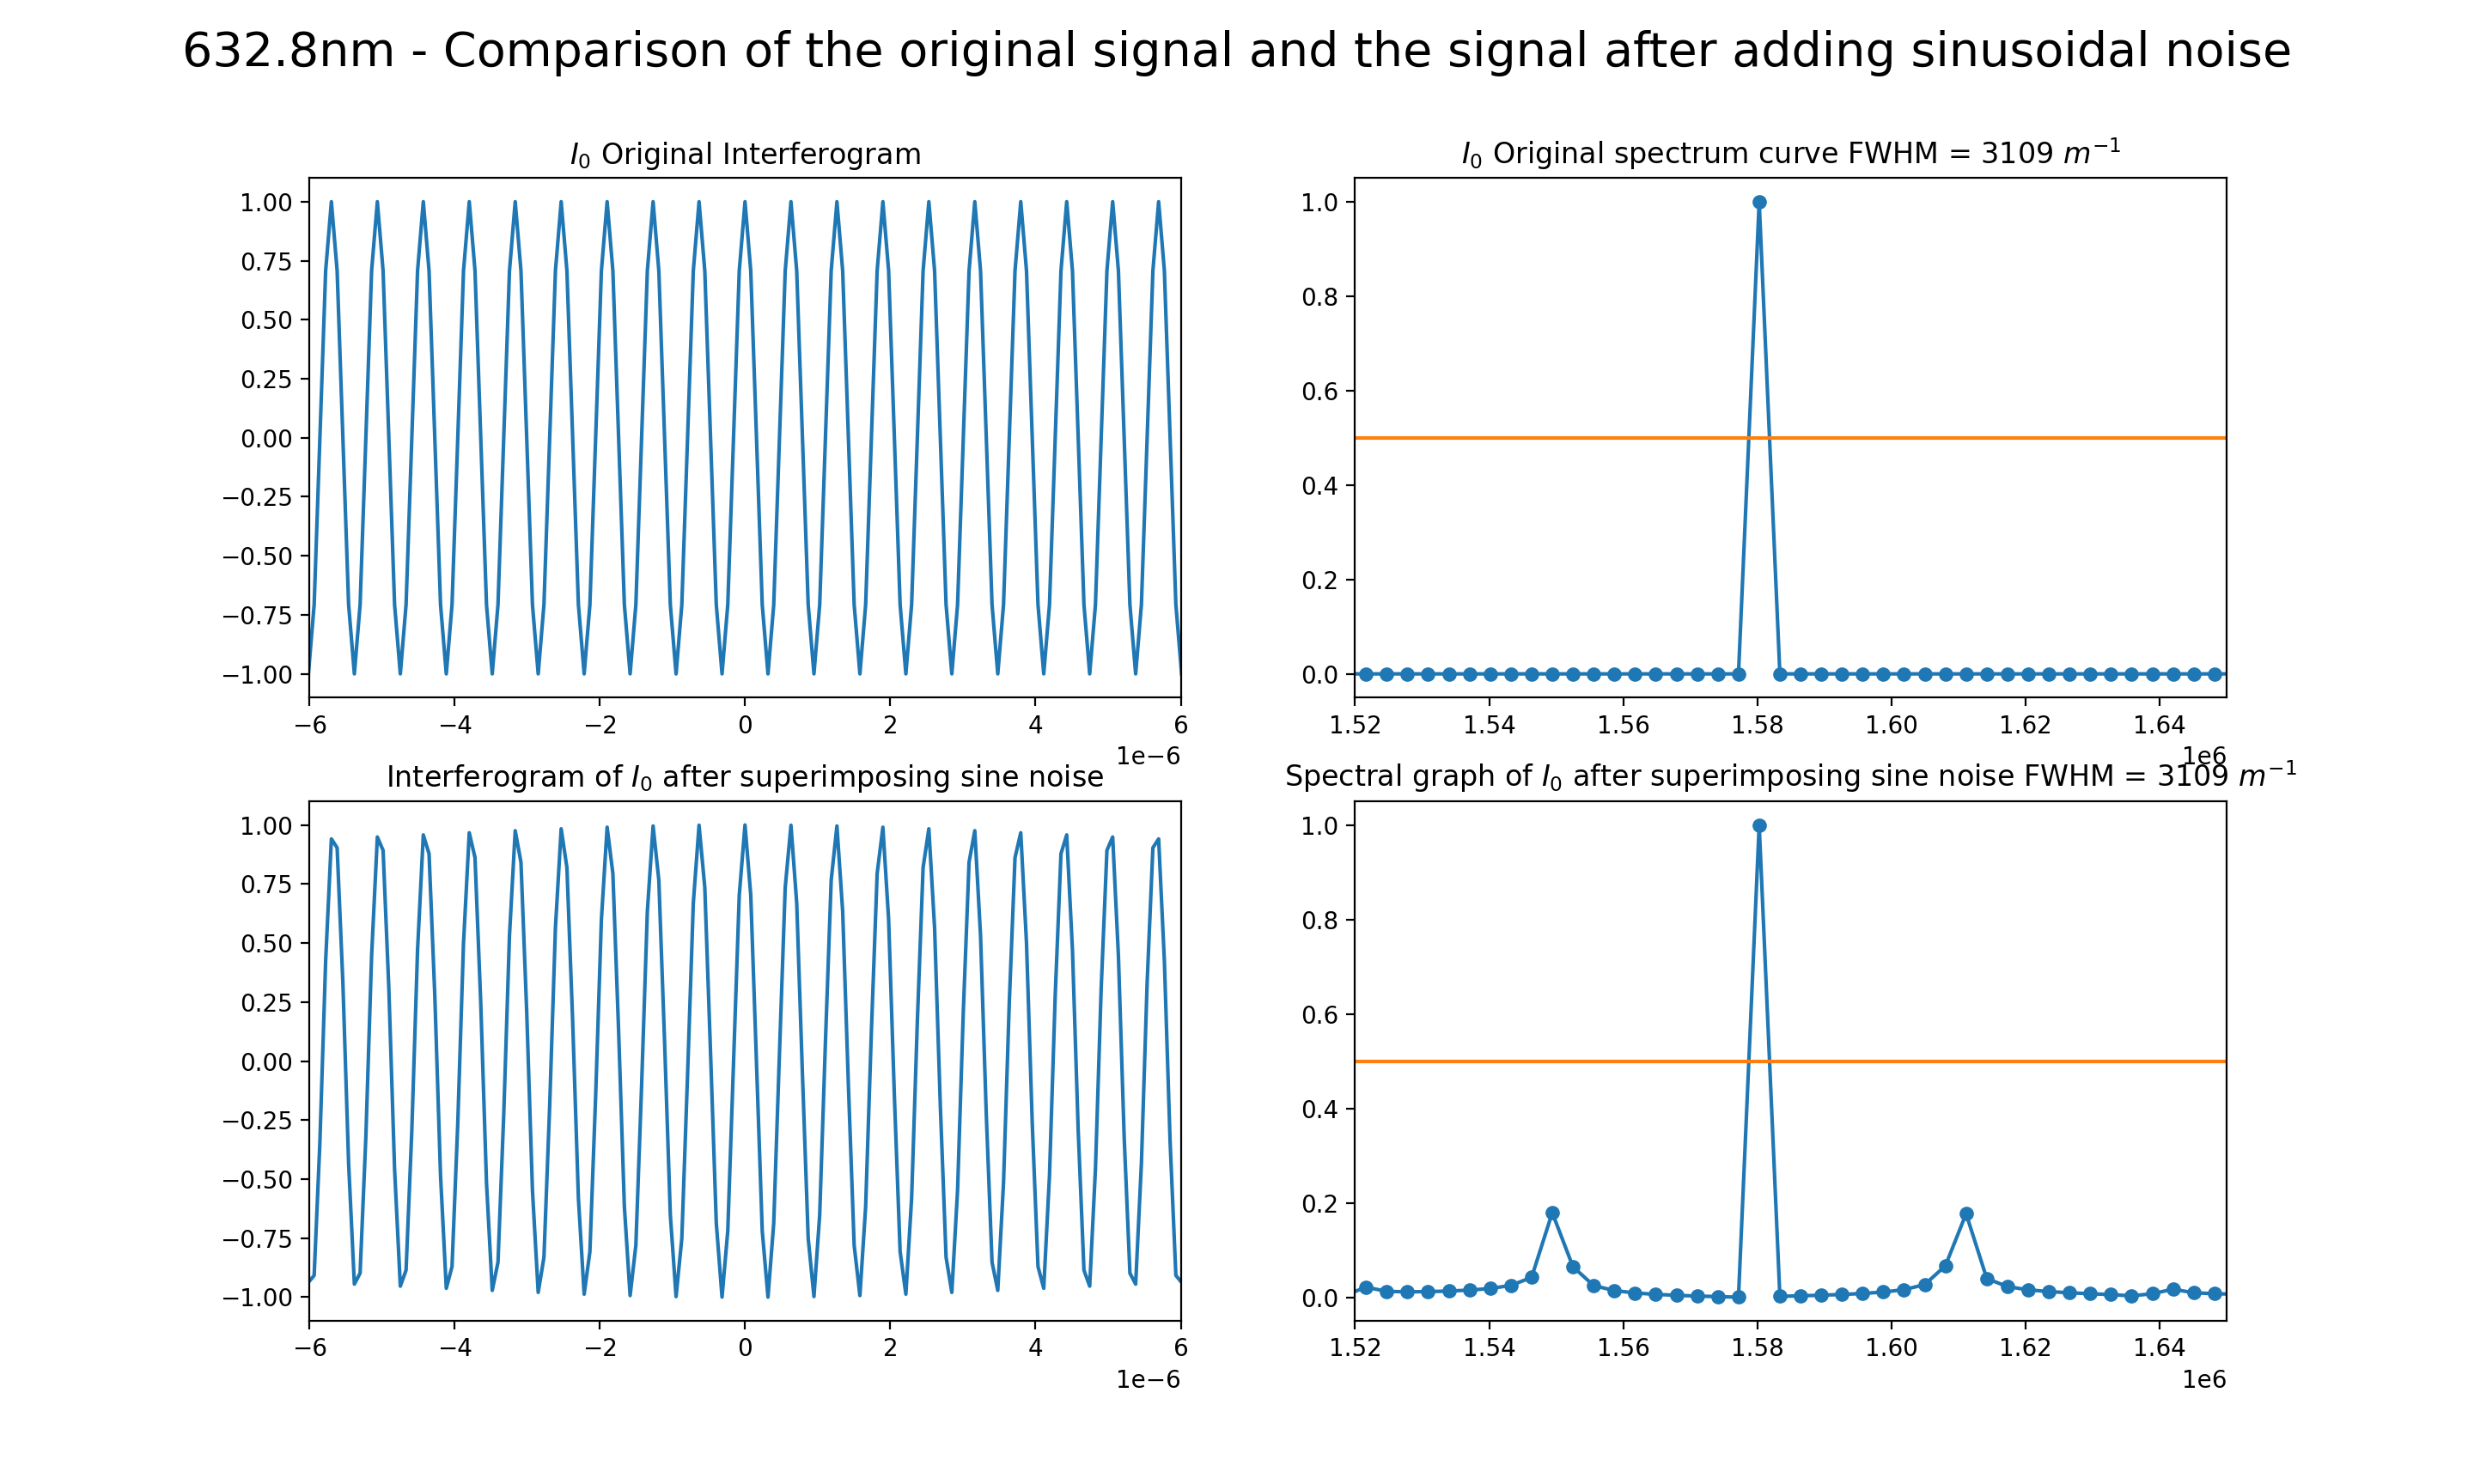
\includegraphics[width=0.5\textwidth]{pic4.png}}
    \caption{正弦噪声叠加结果(图片第一行代表未叠加噪声的干涉图与光谱曲线图,第二行代表添加正弦噪声后的干涉图与光谱曲线图;左半部分代表无噪声干扰与叠加正弦噪声干扰后的干涉图,右半部分代表无噪声干扰与叠加正弦噪声干扰后的光谱曲线图。)}
    \label{pic4}
\end{figure}

\begin{figure}[htbp]
    \centerline{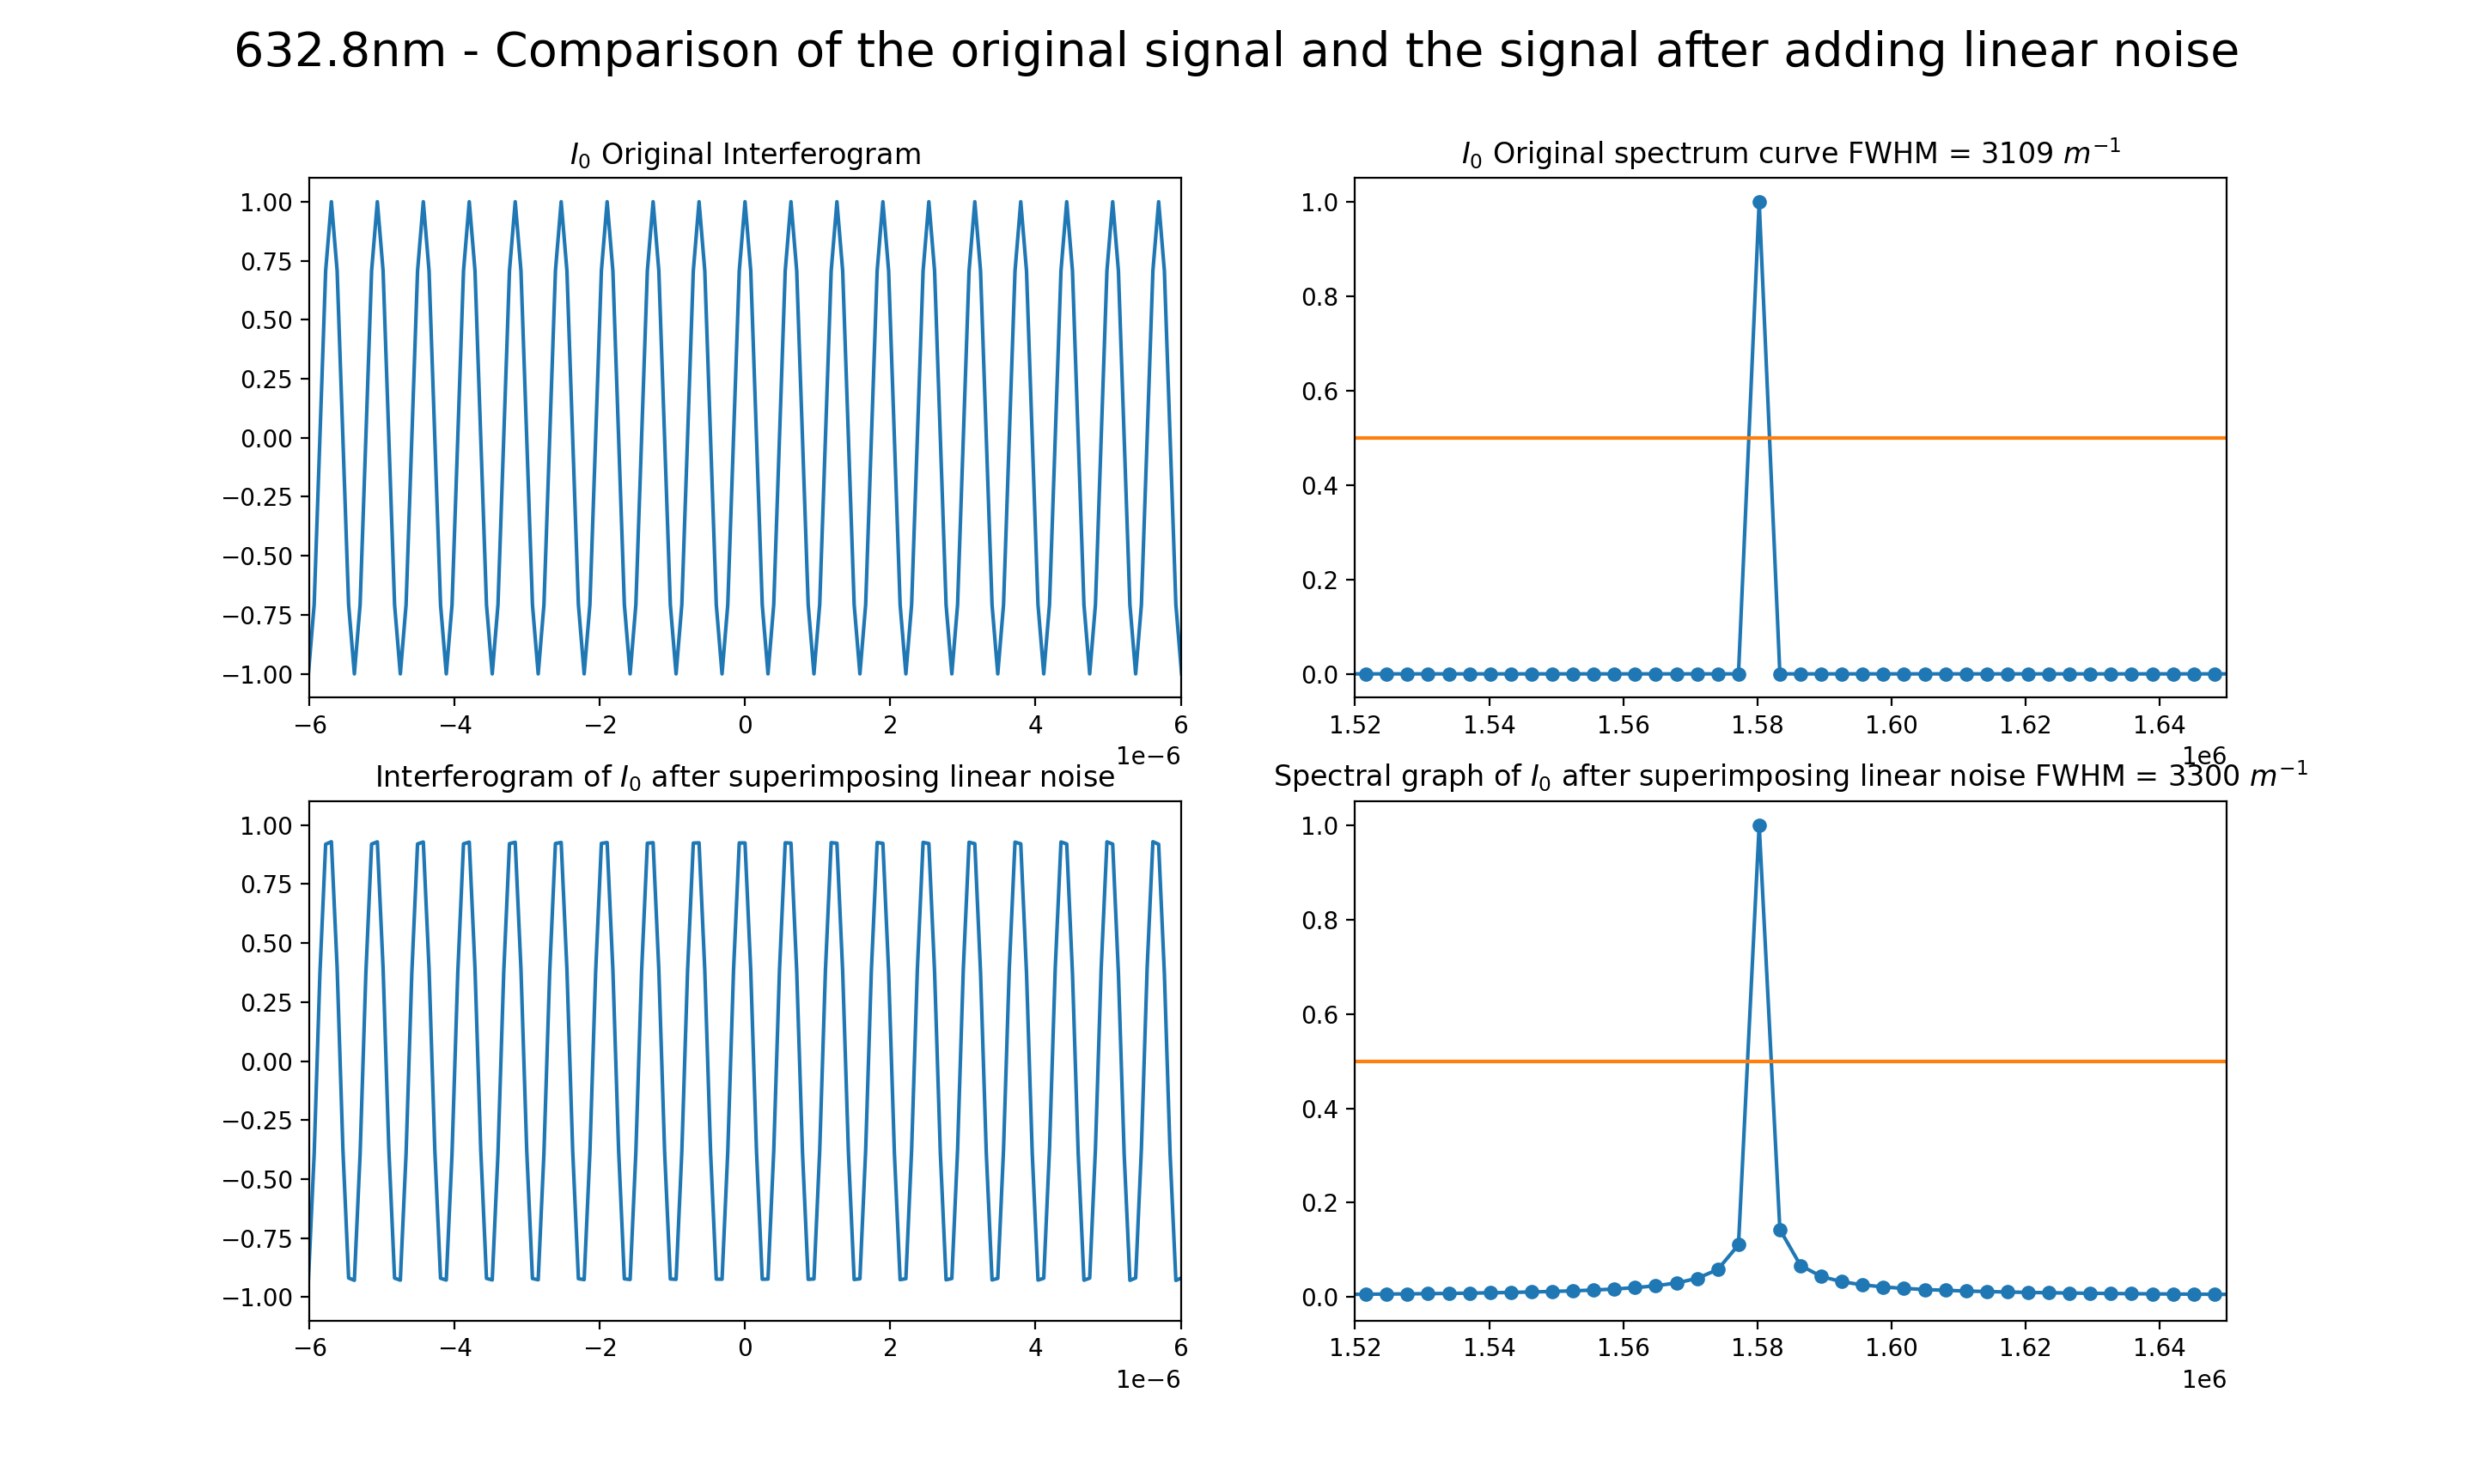
\includegraphics[width=0.5\textwidth]{pic5.png}}
    \caption{随机噪声叠加结果(图片第一行代表未叠加噪声的干涉图与光谱曲线图,第二行代表添加随机噪声后的干涉图与光谱曲线图;左半部分代表无噪声干扰与叠加随机噪声干扰后的干涉图,右半部分代表无噪声干扰与叠加随机噪声干扰后的光谱曲线图。)}
    \label{pic5}
\end{figure}

\begin{figure}[htbp]
    \centerline{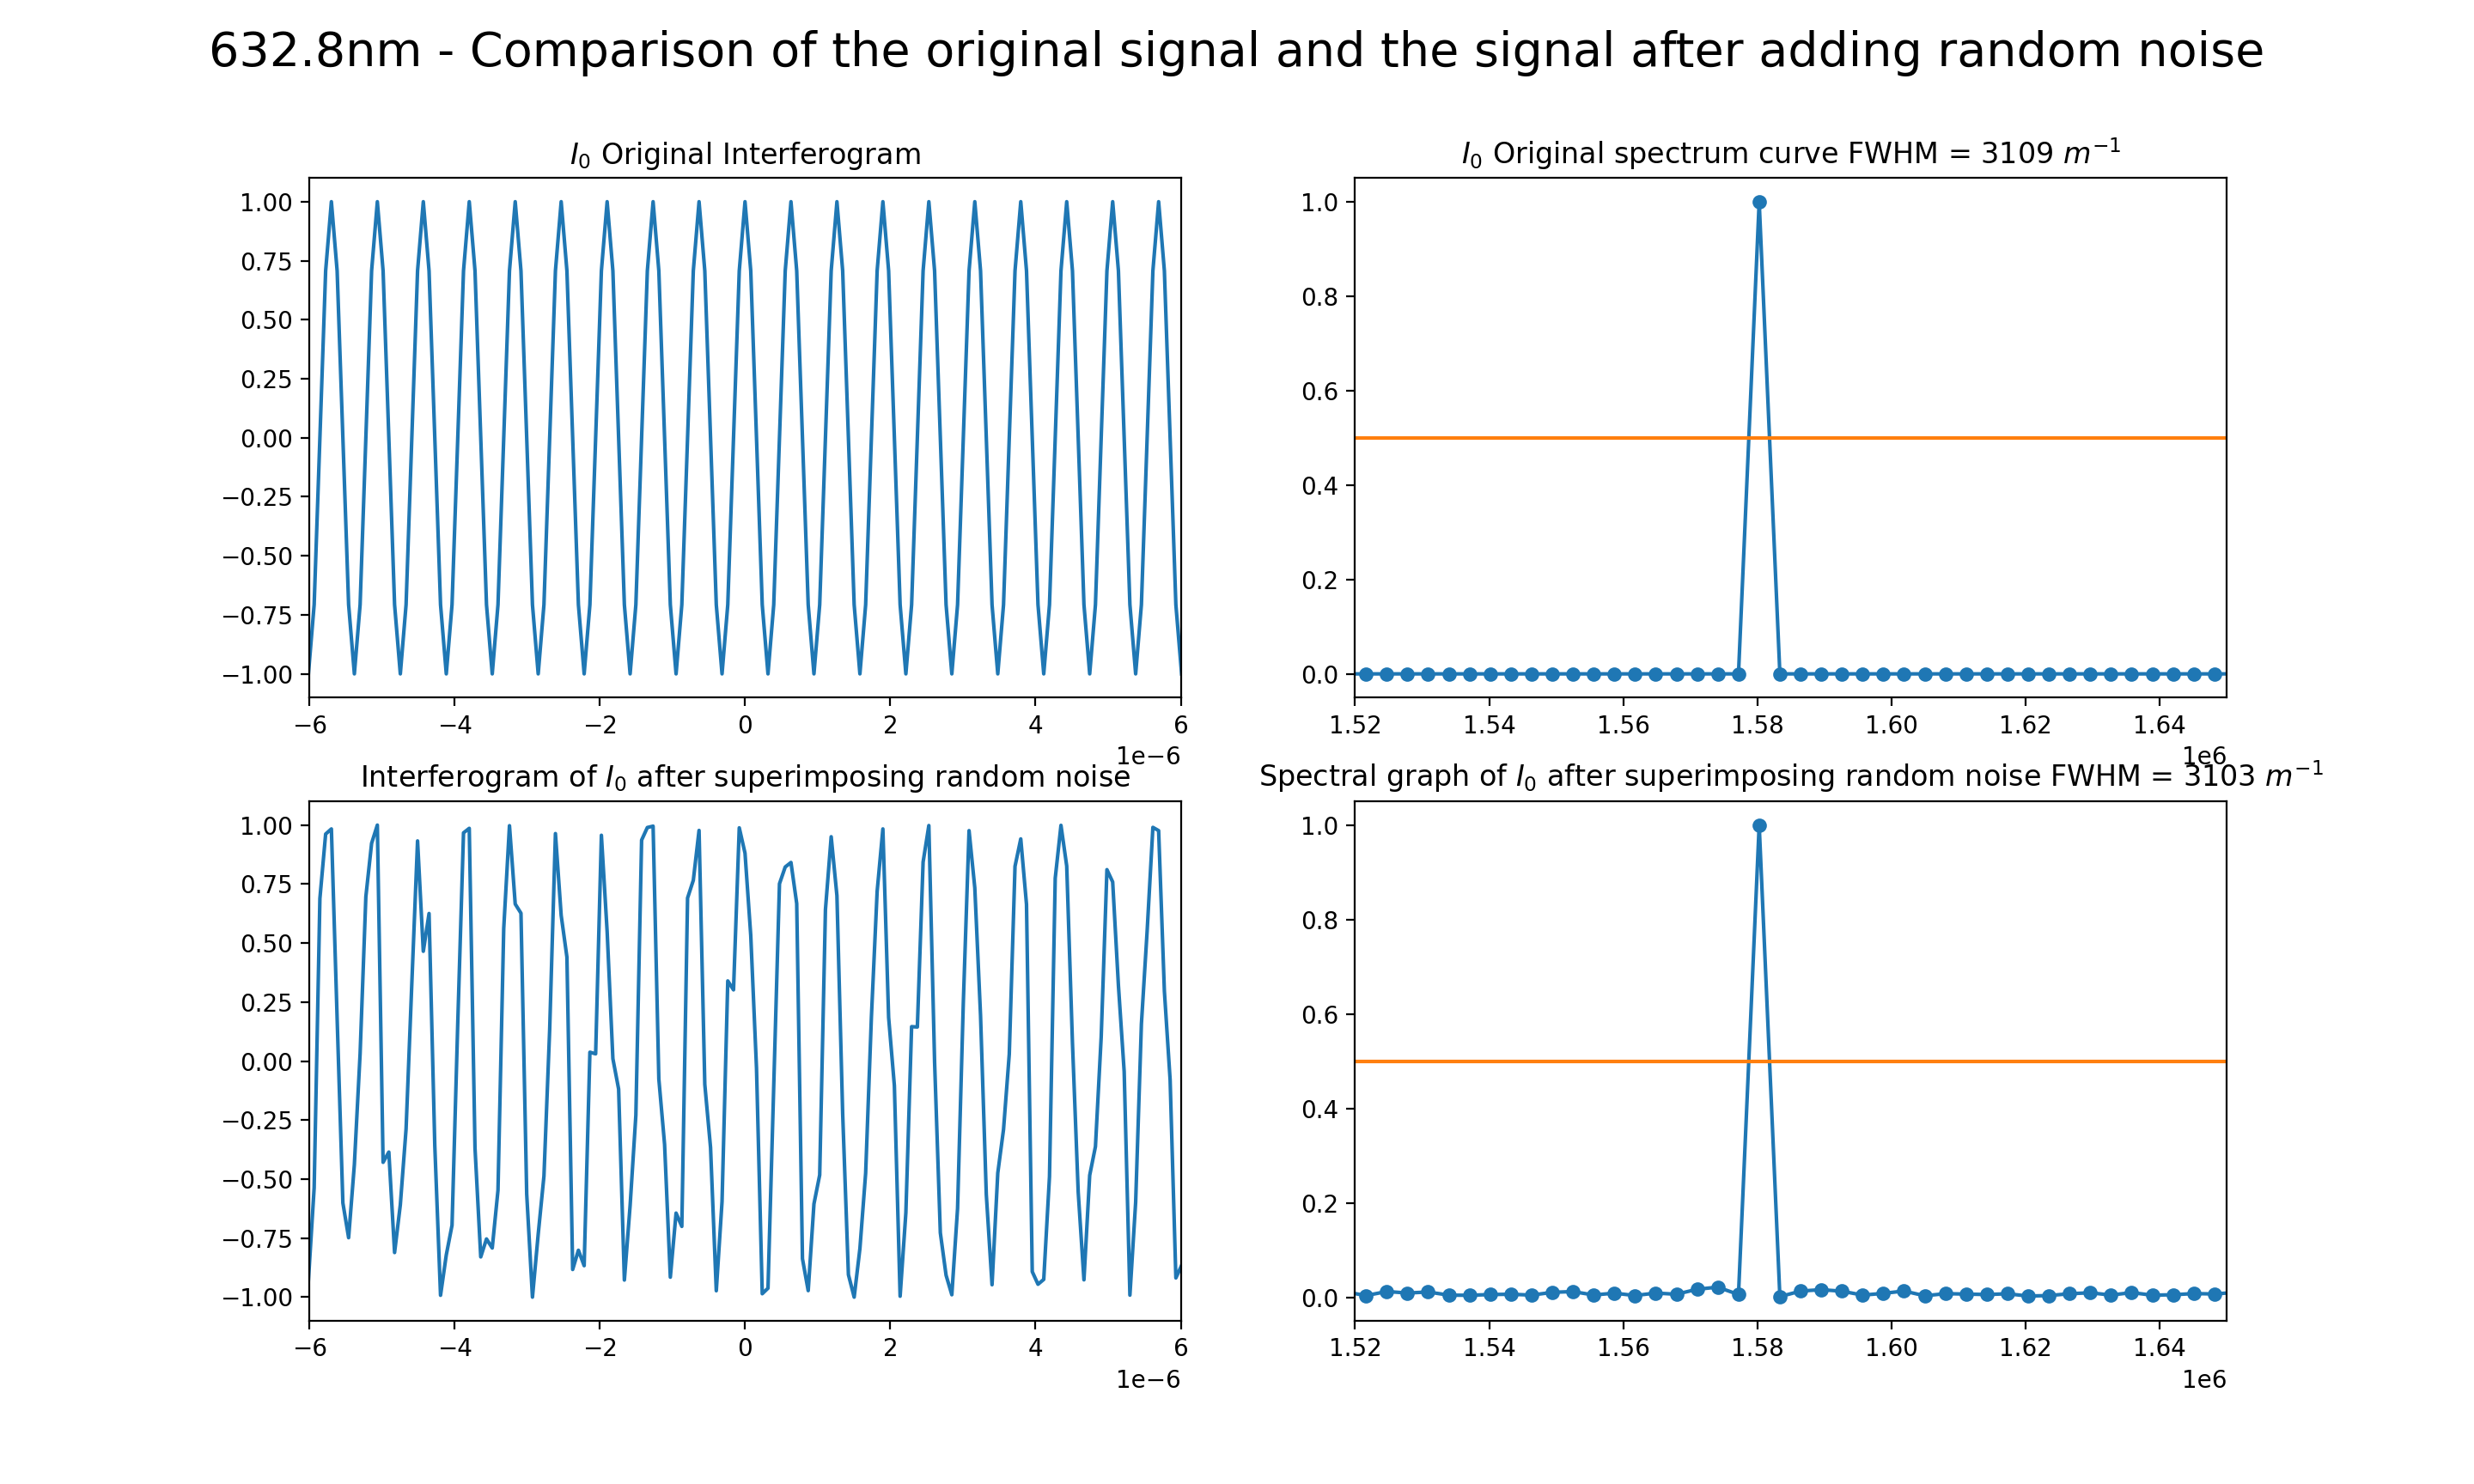
\includegraphics[width=0.5\textwidth]{pic6.png}}
    \caption{线性噪声叠加结果(图片第一行代表未叠加噪声的干涉图与光谱曲线图,第二行代表添加线性噪声后的干涉图与光谱曲线图;左半部分代表无噪声干扰与叠加线性噪声干扰后的干涉图,右半部分代表无噪声干扰与叠加线性噪声干扰后的光谱曲线图。)}
    \label{pic6}
\end{figure}


图片\ref{pic7}将叠加三种不同噪声后的干涉图放在了一起,可以看到,叠加了线性噪声与随机噪声后,原始信号的干涉图变化较大;叠加正弦噪声后的干涉图与原始信号干涉图差别只在幅值上,大体上与原始信号相符合。上述仿真说明线性噪声与随机信号噪声对原始光的干涉图影响较大,叠加正弦噪声对原始光的干涉图影响较小。


图片\ref{pic13}将叠加三种不同噪声后的光谱测量曲线放在了一起,可以看到,叠加了噪声后,原始信号周围出现了小部分的旁瓣,叠加正弦噪声后旁瓣峰值较高,这是由于正弦噪声信号的频谱存在两个幅值不为零的频率点。同时,叠加线性噪声后的光谱测量曲线的半峰全宽与原始信号相比较为宽,而叠加正弦噪声信号与随机信号后光谱测量曲线的半峰全宽与原始信号相比较无明显变化,此现象说明线性噪声会使得原始波形的波形分辨率下降,从频谱上分析即为使得原始光谱测量曲线的半峰全宽变宽。
\begin{figure*}[htbp]
	\centerline{
		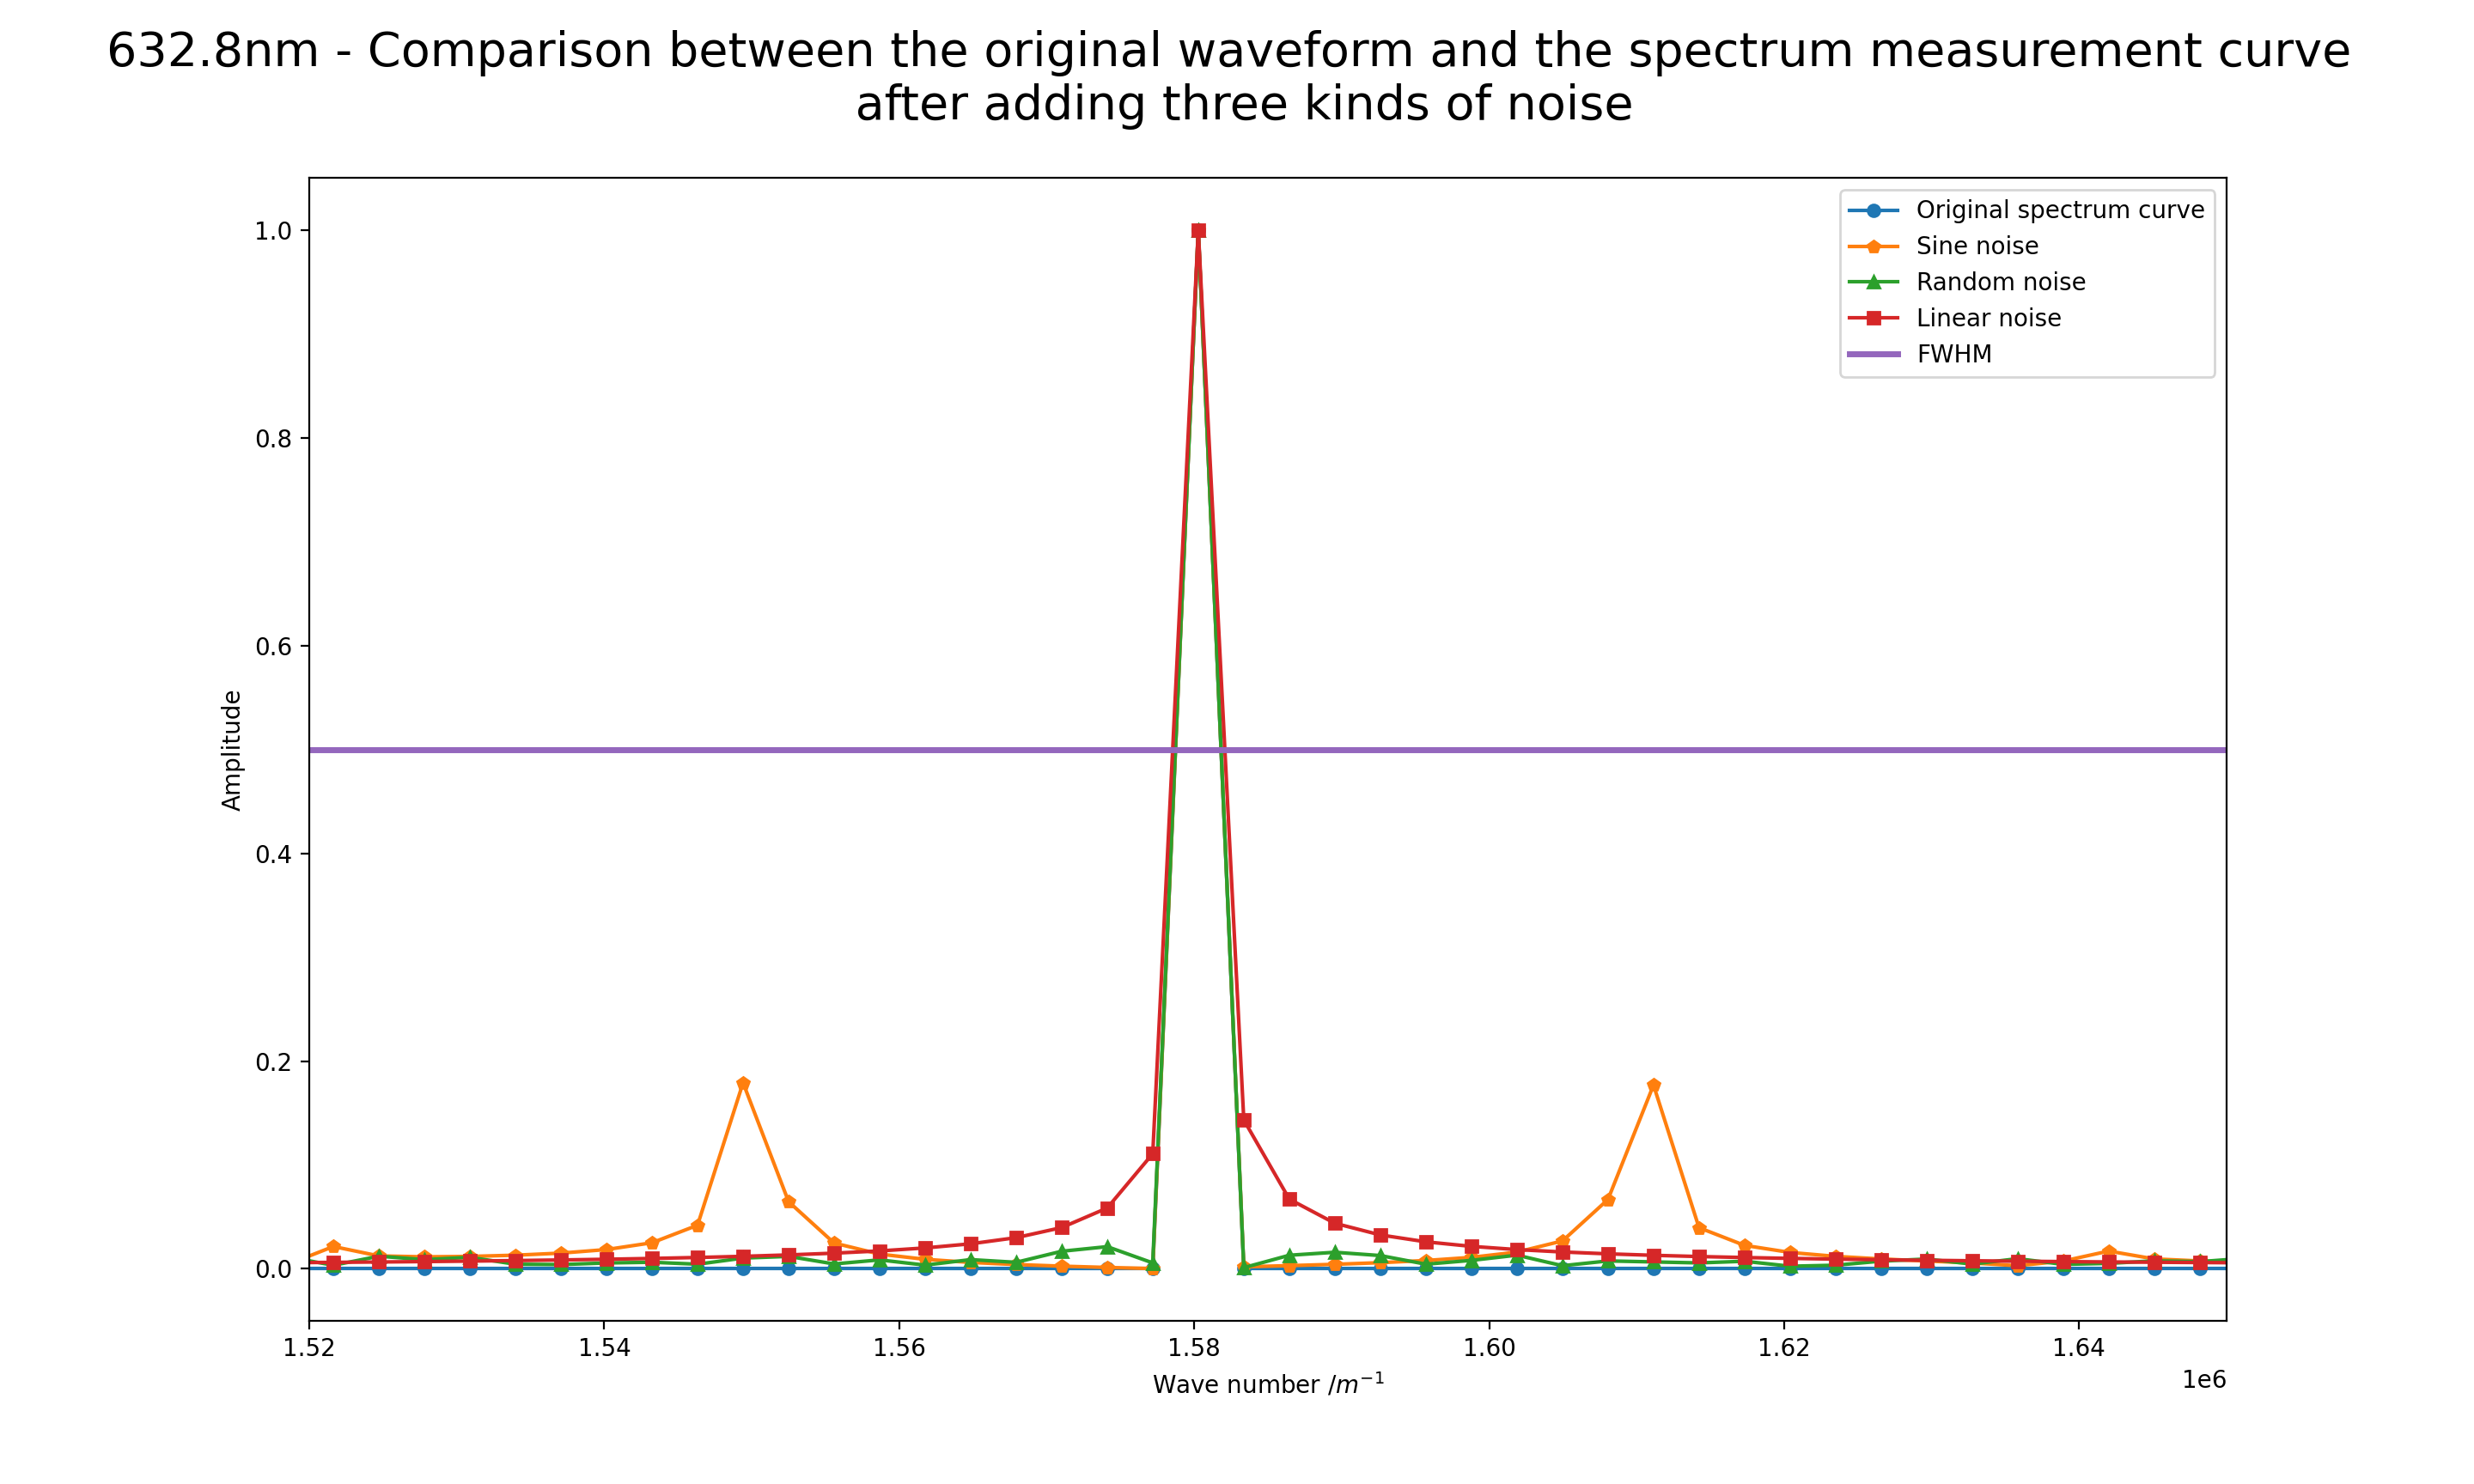
\includegraphics[width=22cm]{pic13.png} 	
	}
	\caption{原始信号的干涉图与叠加三种不同噪声后光谱测量曲线的比较}
	\label{pic13}
\end{figure*}

\section{结语}
本实验完成了利用Python仿真同时考虑有限扫描长度和采样间隔误差两因素影响下的傅里叶变换光谱测量系统的光谱测量曲线。

\appendix[实验代码]
\begin{lstlisting}[language=python]
    import numpy as np
    import matplotlib.pyplot as plt
    from scipy.fftpack import fft
    from pylab import *
    
    # 波长为532nm
    laimda0 = 632.8*10**(-9)
    # 79.1nm的采样间隔 
    i = 79.1*10**(-9)
    # 中心点的采样频
    sigma0 = 1/laimda0
    p1 = (-1)*(2**11)*79.1*10**(-9)
    # 2**n个点 
    p2 = (2**11-1)*79.1*10**(-9)
    # 无补零 
    x0 = np.arange(p1, p2, i)
    n0 = n1 = 2**(int(np.log2(len(x0)))+1)
    print("n0 length = %d" %n0)
    
    ###########################
    #  此部分为叠加正弦噪声
    ###########################
    noise_sin1 = laimda0/16*np.sin(2*np.pi*(3*10**4)*x0)
    
    I0 = np.cos(2*np.pi*sigma0*x0)
    Iw0 = np.cos(2*np.pi*sigma0*(x0 + noise_sin1))
    
    Y0 = 2*abs(fft(I0,n0))
    Y0_max = max(Y0);
    Y0 = Y0/Y0_max
    Y0 = Y0[:int(n0/2)]
    
    Yw0 = 2*abs(fft(Iw0,n0))
    Yw0_max = max(Yw0);
    Yw0 = Yw0/Yw0_max
    Yw0 = Yw0[:int(n0/2)]
    
    # 设置频谱图的横坐标
    fs_0 = 1/i*np.arange(n0/2)/n0
    
    best_Y0_average_range = 0.5*np.ones((Y0.size, 1))
    
    figure(1)
    plt.plot(x0, noise_sin1)
    plt.suptitle("Waveform of sinusoidal noise", fontsize = 25)
    
    figure(2)
    subplot(2,2,1)
    plt.plot(x0, I0)
    plt.xlim(-6*(10**(-6)), 6*(10**(-6)))
    plt.title("$I_0$ Original Interferogram")
    
    
    subplot(2,2,2)
    plt.plot(fs_0, Y0, marker='o', ms=5)
    plt.plot(fs_0,best_Y0_average_range)
    plt.title("$I_0$ Original spectrum curve FWHM = 3109 $m^{-1}$")
    plt.xlim(1.52*(10**6), 1.65*(10**6))
    
    subplot(2,2,3)
    plt.plot(x0, Iw0)
    plt.xlim(-6*(10**(-6)), 6*(10**(-6)))
    plt.title("Interferogram of $I_0$ after superimposing sine noise")
    
    subplot(2,2,4)
    plt.plot(fs_0, Yw0, marker='o', ms=5)
    plt.plot(fs_0,best_Y0_average_range)
    plt.title("Spectral graph of $I_0$ after superimposing sine noise FWHM = 3109 $m^{-1}$")
    plt.xlim(1.52*(10**6), 1.65*(10**6))
    
    plt.suptitle("632.8nm - Comparison of the original signal and the signal after adding sinusoidal noise", fontsize = 20)
    
    ###############################
    #  此部分为叠加随机噪声
    ###############################
    noise_rand = laimda0/5*(rand(1,len(x0)))
    Iw1 = np.cos(2*np.pi*sigma0*(x0 + noise_rand[0]))
    
    Yw1 = 2*abs(fft(Iw1,n0))
    Yw1_max=max(Yw1);
    Yw1 = Yw1/Yw1_max
    Yw1 = Yw1[:int(n0/2)]
    
    # 设置频谱图的横坐标
    fs_1 = 1/i*np.arange(n0/2)/n0
    
    figure(3)
    plt.plot(x0, noise_rand[0])
    plt.suptitle("Waveform of random noise", fontsize = 25)
    
    figure(4)
    subplot(2,2,1)
    plt.plot(x0, I0)
    plt.xlim(-6*(10**(-6)), 6*(10**(-6)))
    plt.title("$I_0$ Original Interferogram")
    
    
    subplot(2,2,2)
    plt.plot(fs_1, Y0, marker='o', ms=5)
    plt.plot(fs_0,best_Y0_average_range)
    plt.title("$I_0$ Original spectrum curve FWHM = 3109 $m^{-1}$")
    plt.xlim(1.52*(10**6), 1.65*(10**6))
    
    subplot(2,2,3)
    plt.plot(x0, Iw1)
    plt.xlim(-6*(10**(-6)), 6*(10**(-6)))
    plt.title("Interferogram of $I_0$ after superimposing random noise")
    
    subplot(2,2,4)
    plt.plot(fs_1, Yw1, marker='o', ms=5)
    plt.plot(fs_0,best_Y0_average_range)
    plt.title("Spectral graph of $I_0$ after superimposing random noise FWHM = 3103 $m^{-1}$")
    plt.xlim(1.52*(10**6), 1.65*(10**6))
    
    plt.suptitle("632.8nm - Comparison of the original signal and the signal after adding random noise", fontsize = 20)
    
    #############################
    #  此部分为叠加线性噪声
    #############################
    noise_linear = linspace(0,i,len(x0))
    Iw2 = np.cos(2*np.pi*sigma0*(x0 + noise_linear))
    
    Yw2 = 2*abs(fft(Iw2,n0))
    Yw2_max=max(Yw2);
    Yw2 = Yw2/Yw2_max
    Yw2 = Yw2[:int(n0/2)]
    
    # 设置频谱图的横坐标
    fs_2 = 1/i*np.arange(n0/2)/n0
    
    figure(5)
    plt.plot(x0, noise_linear)
    plt.suptitle("Waveform of linear noise", fontsize = 25)
    
    figure(6)
    subplot(2,2,1)
    plt.plot(x0, I0)
    plt.xlim(-6*(10**(-6)), 6*(10**(-6)))
    plt.title("$I_0$ Original Interferogram")
    
    
    subplot(2,2,2)
    plt.plot(fs_1, Y0, marker='o', ms=5)
    plt.plot(fs_0,best_Y0_average_range)
    plt.title("$I_0$ Original spectrum curve FWHM = 3109 $m^{-1}$")
    plt.xlim(1.52*(10**6), 1.65*(10**6))
    
    subplot(2,2,3)
    plt.plot(x0, Iw2)
    plt.xlim(-6*(10**(-6)), 6*(10**(-6)))
    plt.title("Interferogram of $I_0$ after superimposing linear noise")
    
    subplot(2,2,4)
    plt.plot(fs_2, Yw2, marker='o', ms=5)
    plt.plot(fs_0,best_Y0_average_range)
    plt.title("Spectral graph of $I_0$ after superimposing linear noise FWHM = 3300 $m^{-1}$")
    plt.xlim(1.52*(10**6), 1.65*(10**6))
    
    plt.suptitle("632.8nm - Comparison of the original signal and the signal after adding linear noise", fontsize = 20)
    
    figure(7)
    l1, = plt.plot(x0, I0)
    l2, = plt.plot(x0, Iw0)
    l3, = plt.plot(x0, Iw1)
    l4, = plt.plot(x0, Iw2)
    plt.legend(handles=[l1, l2, l3, l4],labels=['Original spectrum curve', 'Sine noise', 'Random noise', 'Linear noise'], loc='upper right')
    plt.suptitle("632.8nm - Comparison between the original waveform and \n the waveform after adding three kinds of noise", fontsize = 20)
    plt.xlim(-2*(10**(-6)), 2*(10**(-6)))
    plt.xlabel("Scan Length$/m$")
    plt.ylabel("Interference Intensity")
    
    figure(8)
    s1, = plt.plot(fs_0, Y0, marker='o', ms=5)
    s2, = plt.plot(fs_0, Yw0, marker='p', ms=5)
    s3, = plt.plot(fs_1, Yw1, marker='^', ms=5)
    s4, = plt.plot(fs_2, Yw2, marker='s', ms=5)
    s5, = plt.plot(fs_0,best_Y0_average_range, linewidth = 2.5)
    plt.legend(handles=[s1, s2, s3, s4, s5],labels=['Original spectrum curve', 'Sine noise', 'Random noise', 'Linear noise', 'FWHM'], loc='upper right')
    plt.suptitle("632.8nm - Comparison between the original waveform and the spectrum measurement curve \n after adding three kinds of noise", fontsize = 20)
    plt.xlim(1.52*(10**6), 1.65*(10**6))
    plt.xlabel("Wave number $/m^{-1}$")
    plt.ylabel("Amplitude")
    
    plt.show()
    
\end{lstlisting}

\end{document}
